%\documentclass[12pt,a4paper,oneside]{report}             % Single-side
\documentclass[12pt,a4paper,twoside,openright]{report}  % Duplex

\usepackage[final]{pdfpages}
\usepackage{mathrsfs}
%\PassOptionsToPackage{chapternumber=Huordinal}{magyar.ldf} %betuvel a fejezetek szama
\usepackage{t1enc}
%\usepackage[latin2]{inputenc}
\usepackage{amsmath}
\usepackage{amssymb}
\usepackage{enumerate}
\usepackage{enumitem}

\usepackage[thmmarks]{ntheorem}
\usepackage{graphics}
\usepackage{epsfig}
\usepackage{epstopdf}
\usepackage{listings}
\usepackage{color}
%\usepackage{fancyhdr}
\usepackage{lastpage}
\usepackage{anysize}
\usepackage[magyar]{babel}
\usepackage[utf8]{inputenc}
%\usepackage[T1]{fontenc}
\usepackage{sectsty}
\usepackage{setspace}  % Ettol a tablazatok, abrak, labjegyzetek maradnak 1-es sorkozzel!
\usepackage[hang]{caption}
\usepackage{hyperref}
\usepackage{float} % ezzel lehet helybe rakni az abrat
\usepackage{listings}

\usepackage{subfig}

\usepackage[underline=true,rounded corners=false]{etc/pgf-umlsd}
\usepackage[titletoc]{appendix}
\usepackage{relsize}

\usepackage{array}
\usepackage{multirow}
\usepackage{mdwlist}
\makecompactlist{myitemize*}{itemize}

\usepackage[outerbars,color]{changebar}
\usepackage{todonotes}
\cbcolor{red}

%\usepackage{afterpage}
\usepackage{mathtools}
\DeclarePairedDelimiter\ceil{\lceil}{\rceil}
\DeclarePairedDelimiter\floor{\lfloor}{\rfloor}

%--------------------------------------------------------------------------------------
% Main variables
%--------------------------------------------------------------------------------------
\newcommand{\vikszerzo}{Bakró Nagy István}
\newcommand{\vikkonzulens}{Hartmann Péter\\ Reichardt András}
\newcommand{\vikcim}{Poros plazma kísérletek támogatása multiprocesszoros környezetben}
\newcommand{\viktanszek}{Szélessávú Hírközlés és Villamosságtan Tanszék}
\newcommand{\vikdoktipus}{Diploma}
\newcommand{\vikdepartmentr}{Szélessávú Hírközlés és Villamosságtan Tanszék}

%--------------------------------------------------------------------------------------
% Page layout setup
%--------------------------------------------------------------------------------------
% we need to redefine the pagestyle plain
% another possibility is to use the body of this command without \fancypagestyle
% and use \pagestyle{fancy} but in that case the special pages
% (like the ToC, the References, and the Chapter pages)remain in plane style
\usepackage[left=25mm,right=25mm,top=25mm,bottom=25mm,bindingoffset=10mm]{geometry}
%\pagestyle{plain}
\pagestyle{fancy}
%\setlength{\parindent}{0pt} % áttekinthet?bb, angol nyelv? dokumentumokban
% jellemz? \setlength{\parskip}{8pt plus 3pt minus 3pt} % áttekinthet?bb, angol nyelv? dokumentumokban jellemz?
%\setlength{\parindent}{30pt} % magyar nyelv? dokumentumokban jellemz?
%\setlength{\parskip}{0pt}    % magyar nyelv? dokumentumokban jellemz?

%\marginsize{35mm}{25mm}{25mm}{25mm} % anysize package
%\marginsize{45mm}{45mm}{15mm}{15mm} % anysize package
\setcounter{secnumdepth}{0}
\sectionfont{\large\upshape\bfseries}
\setcounter{secnumdepth}{2}
\singlespacing
\frenchspacing

%--------------------------------------------------------------------------------------
%	Setup hyperref package
%--------------------------------------------------------------------------------------
\hypersetup{
    bookmarks=true,            % show bookmarks bar?
    unicode=true,             % non-Latin characters in Acrobat’s bookmarks
    pdftitle={\vikcim},        % title
    pdfauthor={\vikszerzo},    % author
    pdfsubject={\vikdoktipus}, % subject of the document
    pdfcreator={\vikszerzo},   % creator of the document
    pdfproducer={latex},    % producer of the document
    pdfkeywords={dusty plasma, GPGPU, image processing, OpenCL, particle detecting},    % list of keywords
    pdfnewwindow=true,         % links in new window
    %pdfborder={0 0 0.5 [3 3]},
    colorlinks=true,           % false: boxed links; true: colored links
    linkcolor=blue,           % color of internal links
    citecolor=black,           % color of links to bibliography
    citebordercolor={0 1 0},
    filecolor=black,           % color of file links
    urlcolor=blue,             % color of external links
    breaklinks=true 
}

%--------------------------------------------------------------------------------------
% Set up listings
%--------------------------------------------------------------------------------------

\usepackage{listings}
\usepackage{color}
 
\definecolor{codegreen}{rgb}{0,0.6,0}
\definecolor{codegray}{rgb}{0.5,0.5,0.5}
\definecolor{codepurple}{rgb}{0.58,0,0.82}
\definecolor{backcolour}{rgb}{0.95,0.95,0.92}
\definecolor{lightgray}{rgb}{0.9,0.9,0.9}

\lstset{ %
	language=C++,
	backgroundcolor=\color{backcolour},   
    commentstyle=\color{codegreen},
    keywordstyle=\color{magenta},
    %numberstyle=\tiny\color{codegray},
    stringstyle=\color{codepurple},
    %stringstyle=\scriptsize\sffamily\color{codepurple}, 			% typewriter type for strings
    breakatwhitespace=false,
    breaklines=true,
    captionpos=b,
    keepspaces=true,
    numbers=none,
    numbersep=5pt,
    showspaces=false,
    showstringspaces=false,
    showtabs=false,
    tabsize=5,
	basicstyle=\scriptsize\ttfamily, % print whole listing small
	%keywordstyle=\color{black}\bfseries\underbar, % underlined bold black keywords
	identifierstyle=, 					% nothing happens
	aboveskip=3pt,
	belowskip=3pt,
	columns=fixed,
	backgroundcolor=\color{lightgray},
}

%--------------------------------------------------------------------------------------
%	Some new commands and declarations
%--------------------------------------------------------------------------------------
\newcommand{\code}[1]{{\upshape\ttfamily\scriptsize\indent #1}}
%\renewcommand*{\appendixpagename}{Függelék} 
%\renewcommand*{\appendixtocname}{Függelék} 

% define references
\newcommand{\figref}[1]{\ref{fig:#1}.}
\renewcommand{\eqref}[1]{(\ref{eq:#1})}
\newcommand{\listref}[1]{\ref{listing:#1}.}
\newcommand{\sectref}[1]{\ref{sect:#1}}
\newcommand{\tabref}[1]{\ref{tab:#1}.}


\newcommand{\E}[1]{{\mathop{\bf E\/}\left\{#1\right\}}}
\newcommand{\STD}[1]{{\mathop{\bf STD\/}\left\{#1\right\}}}


\newcommand{\ud}{\ \mathrm{d}}
\newcommand{\mhat}[1]{\mathrm{\hat{#1}}}
\renewcommand{\vec}[1]{\overrightarrow{\mathrm{#1}}}

\DeclareMathOperator*{\argmax}{arg\,max}
%\DeclareMathOperator*[1]{\floor}{arg\,max}
\DeclareMathOperator{\sign}{sgn}
\DeclareMathOperator{\rot}{rot}


\newcommand*{\cleartorightpage}{%
	\clearpage
	\ifodd\value{page}
	\else
		\mbox{}\clearpage
	\fi
}

\renewcommand{\captionlabelfont}{\small\bf}
\renewcommand{\captionfont}{\footnotesize\it}

\author{\vikszerzo}
\title{\viktitle}
%--------------------------------------------------------------------------------------
%	Setup captions
%--------------------------------------------------------------------------------------
\captionsetup[figure]{
%labelsep=none,
%font={footnotesize,it},
%justification=justified,
width=0.8\textwidth,
aboveskip=10pt}


%--------------------------------------------------------------------------------------
% Table of contents and the main text
%--------------------------------------------------------------------------------------
\begin{document}
%\singlespacing

%\pagenumbering{arabic}
%\pagenumbering{roman}
\onehalfspacing
\setcounter{page}{1}
\pagenumbering{roman}
%--------------------------------------------------------------------------------------
%	The title page
%--------------------------------------------------------------------------------------
\begin{titlepage}
\begin{center}

\includegraphics[height=42 mm,keepaspectratio]{figures/eps/BMElogo}\\
\vspace{0.3cm}
\textbf{Budapesti Műszaki és Gazdaságtudományi Egyetem}\\
\textmd{Villamosmérnöki és Informatikai Kar}\\
\textmd{\viktanszek}\\[5cm]

\vspace{0.4cm}
{\huge \bfseries \vikcim}\\[0.8cm]
\vspace{0.5cm}
\textsc{\Large \vikdoktipus}\\[4cm]

\begin{tabular}{cc}
 \makebox[7cm]{\emph{Készítette}} & \makebox[7cm]{\emph{Konzulens}} \\
 \makebox[7cm]{\vikszerzo} & \makebox[7cm]{Hartmann Péter}\\
  & \makebox[7cm]{Reichardt András}
\end{tabular}

\vfill % Whitespace between editor names and publisher logo

\fbox{$\mathscr{BNI}$} \\[0.3\baselineskip] % Publisher logo

\vfill
{\today}
\end{center}
\end{titlepage}
\clearpage


%\setcounter{page}{1}
\pdfbookmark{\contentsname}{toc}
\tableofcontents%\addcontentsline{toc}{chapter}{Tartalomjegyzék}
\clearpage


%--------------------------------------------------------------------------------------
% Nyilatkozat
%--------------------------------------------------------------------------------------
\begin{center}
\large
\textbf{HALLGATÓI NYILATKOZAT}\\
\end{center}

Alulírott \emph{\vikszerzo}, szigorló hallgató kijelentem, hogy ezt a diplomatervet meg nem engedett segítség nélkül, saját magam
készítettem, csak a megadott forrásokat (szakirodalom, eszközök stb.) használtam fel.
Minden olyan részt, melyet szó szerint, vagy azonos értelemben, de átfogalmazva más forrásból átvettem, egyértelműen, a forrás
megadásával megjelöltem.

Hozzájárulok, hogy a jelen munkám alapadatait (szerző(k), cím, angol és magyar nyelvű tartalmi kivonat, készítés éve,
konzulens(ek) neve) a BME VIK nyilvánosan hozzáférhető elektronikus formában,
a munka teljes szövegét pedig az egyetem belsõ hálózatán keresztül (vagy autentikált felhasználók számára) közzétegye.
Kijelentem, hogy a benyújtott munka és annak elektronikus verziója megegyezik.
Dékáni engedéllyel titkosított diplomatervek esetén a dolgozat szövege csak 3 év eltelte után válik hozzáférhetővé.

\begin{flushleft}
\vspace*{1cm}
Budapest, \today
\end{flushleft}

\begin{flushright}
 \vspace*{1cm}
 \makebox[7cm]{\rule{6cm}{.4pt}}\\
 \makebox[7cm]{\emph{\vikszerzo}}\\
 \makebox[7cm]{hallgató}
\end{flushright}

\vfill
%\thispagestyle{empty} % an empty page

\cleartorightpage
%--------------------------------------------------------------------------------------
% Feladatkiiras (a tanszeken atveheto, kinyomtatott valtozat)
%--------------------------------------------------------------------------------------
% \chapter*{Feladatkiírás}
\phantomsection
\addcontentsline{toc}{chapter}{Feladatkiírás}

% A modern alacsony hőmérsékletű plazmafizikai kísérletek egy új, érdekes és izgalmas területe a poros plazmák
% kutatása. Egy elektromos gázkisülésbe helyezett apró (mikrométer méretű) szilárd szemcse a kisülési plazma
% atomi részecskéivel kölcsönhatva elektromosan feltöltődik. A sok töltött szemcséből kialakuló elrendezésben a
% szilárdtestfizikai jelenségek széles spektruma figyelhető meg, pl. kristályrács kialakulása, fázisátalakulás,
% diszlokációk dinamikája, transzport folyamatok, stb. Poros plazmákat jelenleg leginkább alapkutatásokban
% alkalmaznak, de jelentőségük az elektronikai gyártásban, fúziós
% reaktorok üzemeltelésében, {\color{red} terahertz}
% technológiában egyre inkább előtérbe kerül.
% 
% A kísérleti adatgyűjtés és feldolgozás nagyrésze részecske-követő velocimetrián (particle tracking velocimetry)
% alapul, vagyis első lépésben egy nagysebességű kamera segítségével nagyfelbontású képek készülnek, amely
% képek segítségével a porszemcsék pontos (a kamera felbontásánál pontosabb) koordinátáit kell meghatározni. A
% képek elemzése ezidáig csak a mérést követően, hosszú idő alatt volt megvalósítható a vizsgálandó nagy
% adatmennyiség miatt. A multiprocesszoros környezetek segítségével a feldolgozás gyorsítása lehetséges akár
% több nagyságrenddel is.
% 
% A jelölt feladata, hogy a meglévő kísérleti elrendezés, amely az MTA Wigner Fizikai Kutatóközpont
% Szilárdtestfizikai és Optikai Intézezetben található, kiegészítésével a mérés közbeni feldolgozással a mérést
% segítő analízist hajtson végre. Ennek eredményével a mérés előkészítése és elvégzése lényegesen gyorsulhatnak.
% 
% \begin{flushleft}
% \textbf{A jelölt feladata}
% 
% \begin{itemize}
% 	\item Mutassa be a mérési elrendezést és elemezze a kapott adatokat! (Mutassa
% 	be a mérést!)
% 	\item Elemezze a lehetséges multiprocesszoros környezeteket, a feladat
% 	szempontjából lényeges paraméterek és feladatvégrehajtási elvárások szempontjából!
% 	\item Készítsen programot, amely az azonnali (valós idejű) analízisben résztvevő paramétereket számítja ki, a
% 	multiprocesszoros környezet kihasználása nélkül!
% 	\item Készítsen programot, amely a mérési környezetbe illeszkedve a mérésnél
% 	valós időben képes a vizsgált paraméterek megjelenítésére! Mutassa be és
% 	elemezze az elkészített programot!
% 	\item Hasonlítsa össze a multiprocesszoros és a nem-multiprocesszoros
% 	környezetre elkészített programokat erőforrás igény illetve egyéb paraméterek szempontjából!
% \end{itemize}
% \end{flushleft}
% 
% \begin{flushleft}
% \textbf{Irodalom}:
% \begin{itemize}
% 	\item \cite{Hartmann2010} Hartmann P, et. al. ; “Crystallization Dynamics of a Single Layer Complex Plasma”;
% 	Phys. Rev. Lett., 105 (2010) 115004
% 	\item \cite{Hartmann2013} Hartmann P, et. al. ; “Magnetoplasmons in Rotating Dusty	Plasmas”, Phys.	Rev. Lett.
% 	111, 155002 (2013)
% 	\item \cite{HartmannP2013} Hartmann P, Donkó I, Donkó Z; “Single exposure three-dimensional imaging of dusty
% 	plasma clusters”; Rev. Sci. Instrum., 84 (2013) 023501/1-5;
% \end{itemize}
% \end{flushleft}
% 
% \begin{flushleft}
% \vspace*{1cm}
% \textbf{Tanszéki konzulens}: Reichardt András, egy. tanársegéd\\
% \textbf{Külső konzulens}: Hartmann Péter, PhD., tud. főmunkatárs (MTA Wigner FK, SZFKI)
% \end{flushleft}
% 
% 
% 
% \begin{flushleft}
% \vspace*{1cm}
% Budapest, 2014.03.10.
% \end{flushleft}

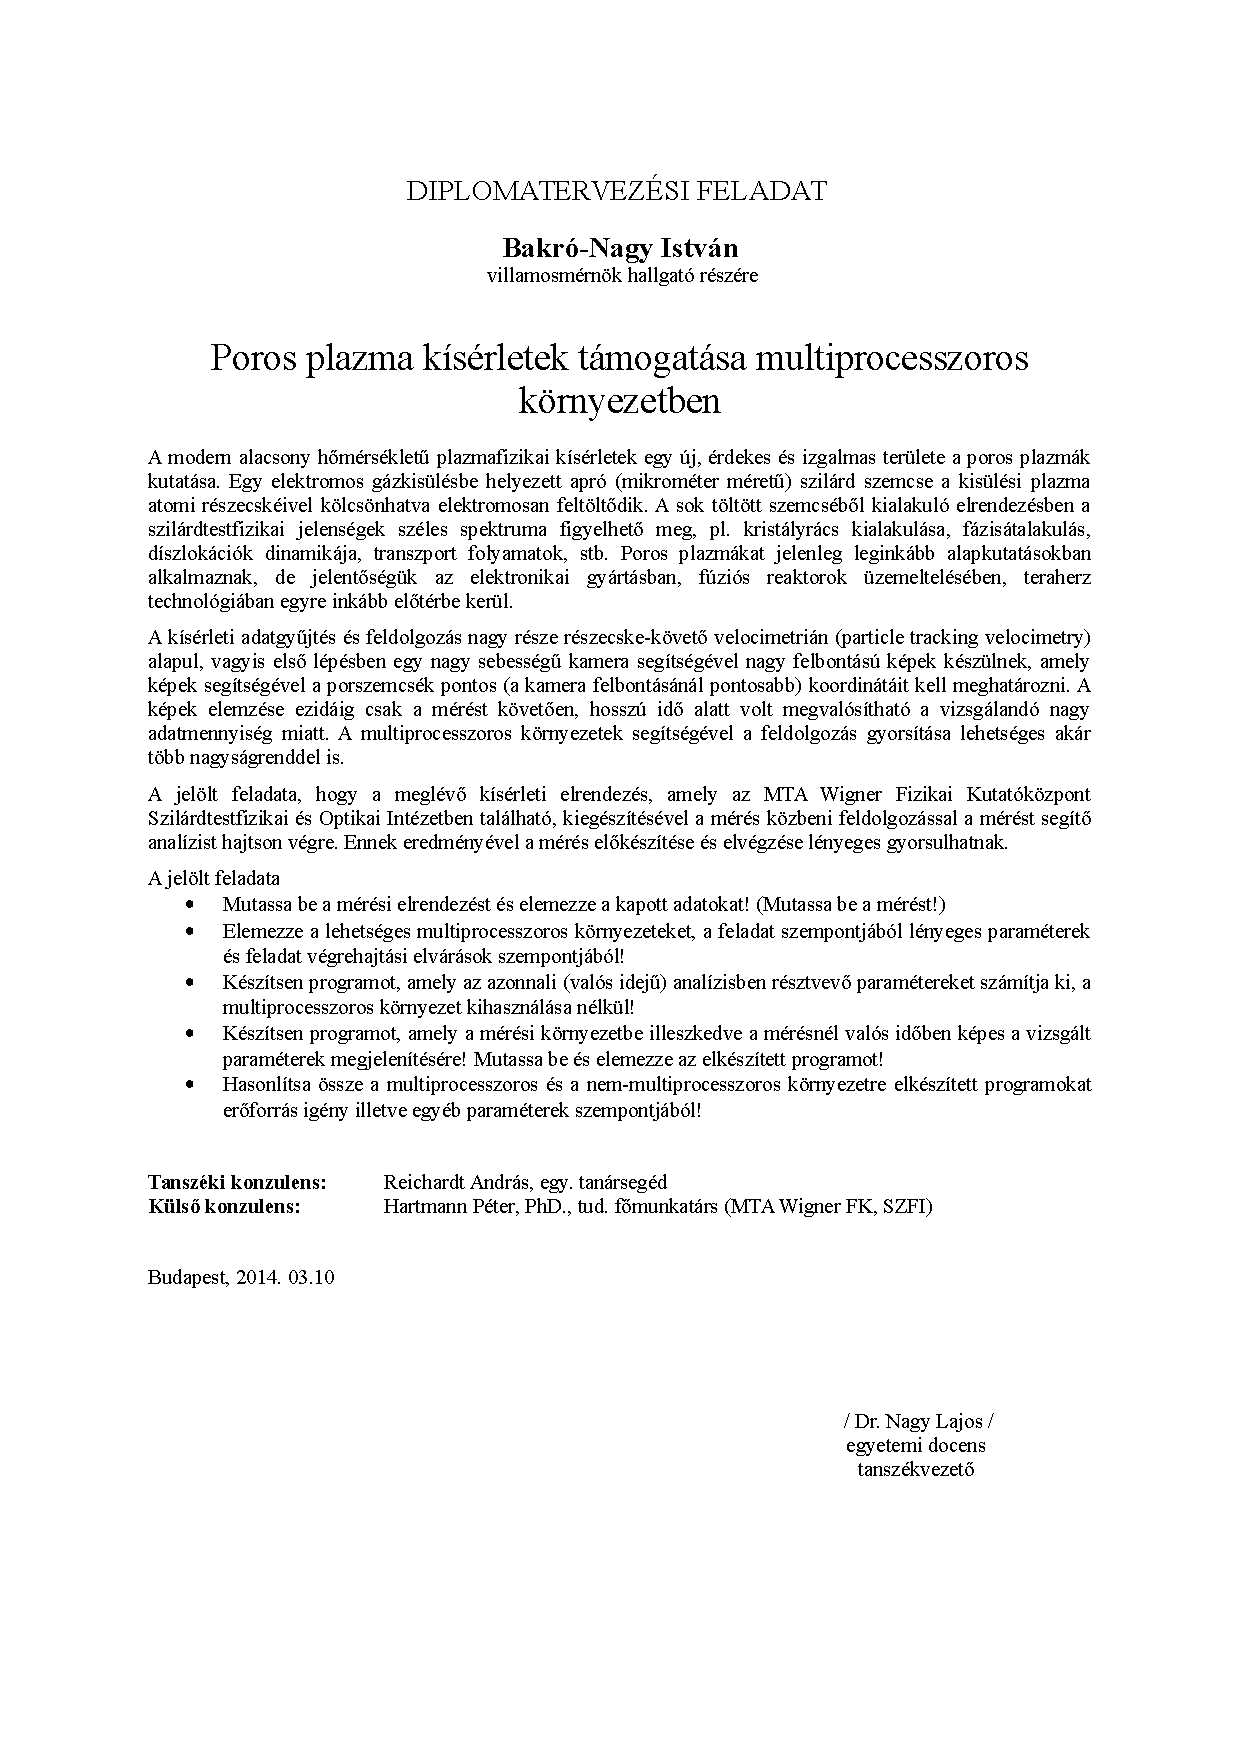
\includepdf[pages={1}]{kiiras.pdf}


%----------------------------------------------------------------------------
% Abstract in hungarian
%----------------------------------------------------------------------------
\chapter*{Kivonat}\addcontentsline{toc}{chapter}{Kivonat}

	hablaty



\chapter*{Abstract}\addcontentsline{toc}{chapter}{Abstract}

	what? what? in the butt
	

\cleartorightpage
\pagenumbering{arabic}
\setcounter{page}{1}

%----------------------------------------------------------------------------
\chapter{A poros plazma kísérlet}
%----------------------------------------------------------------------------

	A poros plazma kísérlet ionizált nemesgáz és az abba szórt porrészecskék megfigyeléséből áll.
	Adott alacsony nyomású gáz terében elhelyezett elektródákra kapcsolt váltakozó feszültséggel 
	lehetséges plazmát létrehozni. A váltakozó villamos tér a töltéssel rendelkező elektronokra 
	olyan erővel hat, hogy azok leszakadnak az atomról ezzel ionizálva azokat.
	A leszakadó elektronok a térben szabadon a ráható erőknek megfelelően mozognak.
	Ez makroszkópikus skálán a gáz vezetővé válását jelenti. A szabad elektronok mozgásának
	során az ionizált atomokon szórodnak, ami ködfénykisüléshez vezet. 
	
	A kísérlet során az előbb ismertett plazma terébe porrészecskéket szórunk. A porrészecskék alatt
	$10nm - 100\mu m$ nagyságú részecskéket értünk, például $SiO_2$, $Al_2O_3$ vagy 
	melamine-formaldehyde-t. A porrészecskék a plazmával interakcióba lépve negatívan feltöltődnek.
	A porrészecskék töltésének és tömegének hányadosa a szabad elektronokhoz és az ionokhoz képest
	sokkal kissebb, ezáltal a mozgására való hatása elhanyagolható.
	
	A porrészecskék transzportjának megértéséhez szükséges a ráható erők azonosítása.
	A különféle erők nagysága a porrészecskék nagyságától különféleképpen skálázódik. Elhanyagolásokat
	ennek megfelelően tehetünk.
	\begin{description}
		\item[Gravitációs $F_g$ erő:] Mikrogravitációban végzett kísérletek és nanométer nagyságú részecskék esetén
			elhanyagolhatóak, de a jelen esetben használt mikrométer nagyságú részecskék esetén dominánsak,
		\item[Villamos tér keltette $F_e$ erő:] A porrészecske töltésével és a villamos tér nagyságával
			arányos. A megfelelően irányított villamos térrel lehetséges a részecskék levitációja,  
		\item[Háttératomon való szóródás $F_n$:] A porrészecske driftje során a háttératomokkal való
			szóródásának makroszkópikus erőként való számításba vétele,
		\item[Hőmérséklet gradiensi $F_{th}$ erő:] A gáz hőmérsékletének gradiense okozta
			gázatomok diffúzív jellegű mozgása által okozott indirekt erőhatás,
		\item[Ion sodrási $F_i$ erő:] Az ionokra ható villamos tér okozta erőnek indirekt hatása a
			porrészecskékre.
	\end{description}
	A poros plazma analízise során fontos szerepet játszik a porrészecskék csatolása.
	A csatolást gyengének és erősnek kategorizáljuk aszerint, hogy a részecskék szomszédja általi
	átlagos potenciális energia az átlagos termikus (kinetikus) energiájához képest kissebb vagy
	nagyobb.
	A csatolást a Coulomb csatolási paraméterrel ($\Gamma$) lehet számosítani, ami a szomszédos
	részecskék Coulomb potenciáljának és termikus energiájának hatványa:
	\begin{equation}
		\Gamma = \cfrac{Q^2 / 4\pi\varepsilon_0 d}{kT_d} 
	\end{equation}
	ahol $Q$ a részecskék töltése, $d$ az átlagos részecske távolság és a $T_d$ a por hőmérséklete.
	Ha a $\Gamma$ értéke egy kritikus érték fölé $\Gamma > 150$ növekszik, akkor
	Ikawa jóslata szerint a porrészecskék Coulomb kristályszerkezetbe rendeződik.
	
	Az iparban anyag porlasztására és mintázat maratására használják. Továbbá szennyeződésként a VLSI
	áramkörök gyártásakor jelentkezik, ami a kihozatal csökkenését és a teljesítmény csökkenéséhez
	vezet. Laboratóriumi környezetben kristály halmazállapot változását, viszkozitását lehet kutatni. 

%----------------------------------------------------------------------------
\section{A kísérlet}
%----------------------------------------------------------------------------
	A kísérlet lebonyolítására egy speciális kamrára van szükség, amiben lehetséges a plazma
	létrehozása, a porrészecskék szórása illetve a megfelelő villamos tér létrehozása.
	A kamrának hermetikusan jól zártnak kell lennie, hogy csak a kívánt gázt tartalmazza.
	A középvákuumú működéshez kétlépéses vákuumszivattyút kell alkalmazni.
	
	
	A kamra sematikus ábrája a \ref{fig:meresch}. ábrán látható.
	A porrészecskék levitációjáért a villamos tér felelős. A síkba való zárás parabolikus
	potenciállal lehetséges. Az ilyen tér létrehozása a következő elektróda elrendezéssel lehetséges:
	alul elhelyezett korong alakú elektróda, ami felett egy gyűrű alakú elektróda helyezkedik el.
	Az ilyen elektródarendszerre kapcsolt váltakozó feszültség a beszórt porrészecskéket lebegtetni
	tudja. Továbbá a részecskék követéséhez azokat lézerrel megvilágítjuk és nagysebességű kamerával
	felvételt készítünk róla.
	
	\begin{figure}[H]
		\centering
		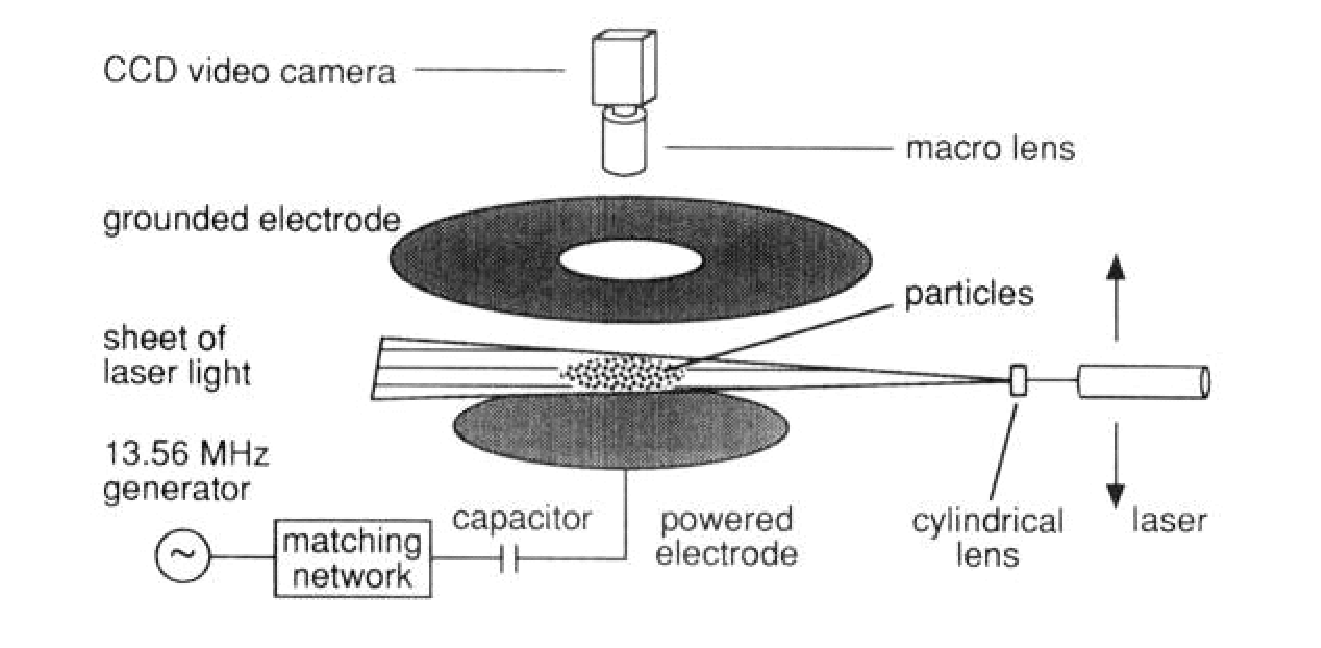
\includegraphics[width=0.9\columnwidth]{figures/eps/dust_camera.eps}
		\caption[A mérési elrendezés sematikus ábrája]{A mérési elrendezés sematikus ábrája (forrás: \cite{Merlino2006})} 
		\label{fig:meresch}
	\end{figure}
	
	A kamrát (\ref{fig:kamra}. ábra) Hartmann Péter külső konzulensem építette és a MTA Wigner FK SZFI
	Gázkisülési Laboratóriumában található.
	
	\noindent A paraméterei:
	\begin{myitemize*}
		\item Kamra belső átmérője: $25cm$
		\item Kamra belső magassága: $18cm$
		\item Alsó elektróda átmérője: $18cm$
		\item Felső gyűrű elektróda belső átmérője: $15cm$
		\item Felső elektróda távolsága az alsótól: $13cm$
		\item Argon gáz nyomása: $1.2\pm0.05 Pa$
		\item Gáz átfolyása: $\sim 0.01 CCPM$
		\item RF gerjesztés: $7W\ @ \ 13.56 MHz$
		\item Porrészecske: melamine-formaldehyde
		\item Porrészecske átmérője: $4.38\pm 0.06 \mu m$
		\item Porrészecske tömege. $6.64\cdot10^{-14} kg$
		\item Látható porrészecskék száma: $\sim 2500$
		\item Megvilágító lézer: $200mW\quad @ \quad 532nm$
		\item Kamera: $1.4 MPixel\ @\ 100 FPS$
	\end{myitemize*}
	A kamra alsó elektródáját lehetséges egy motorral forgásba hozni. Az elektróda felületének érdessége által a kamrában
	lévő gáz is forgásba jön. A gáz forgása az $F_i$ ionsodrási erővel hat a porrészecskékre.
	A forgó rendszert nagy mágneses tér Lorentz erejének feleltethető meg.
	\begin{figure}[H]
		\centering
		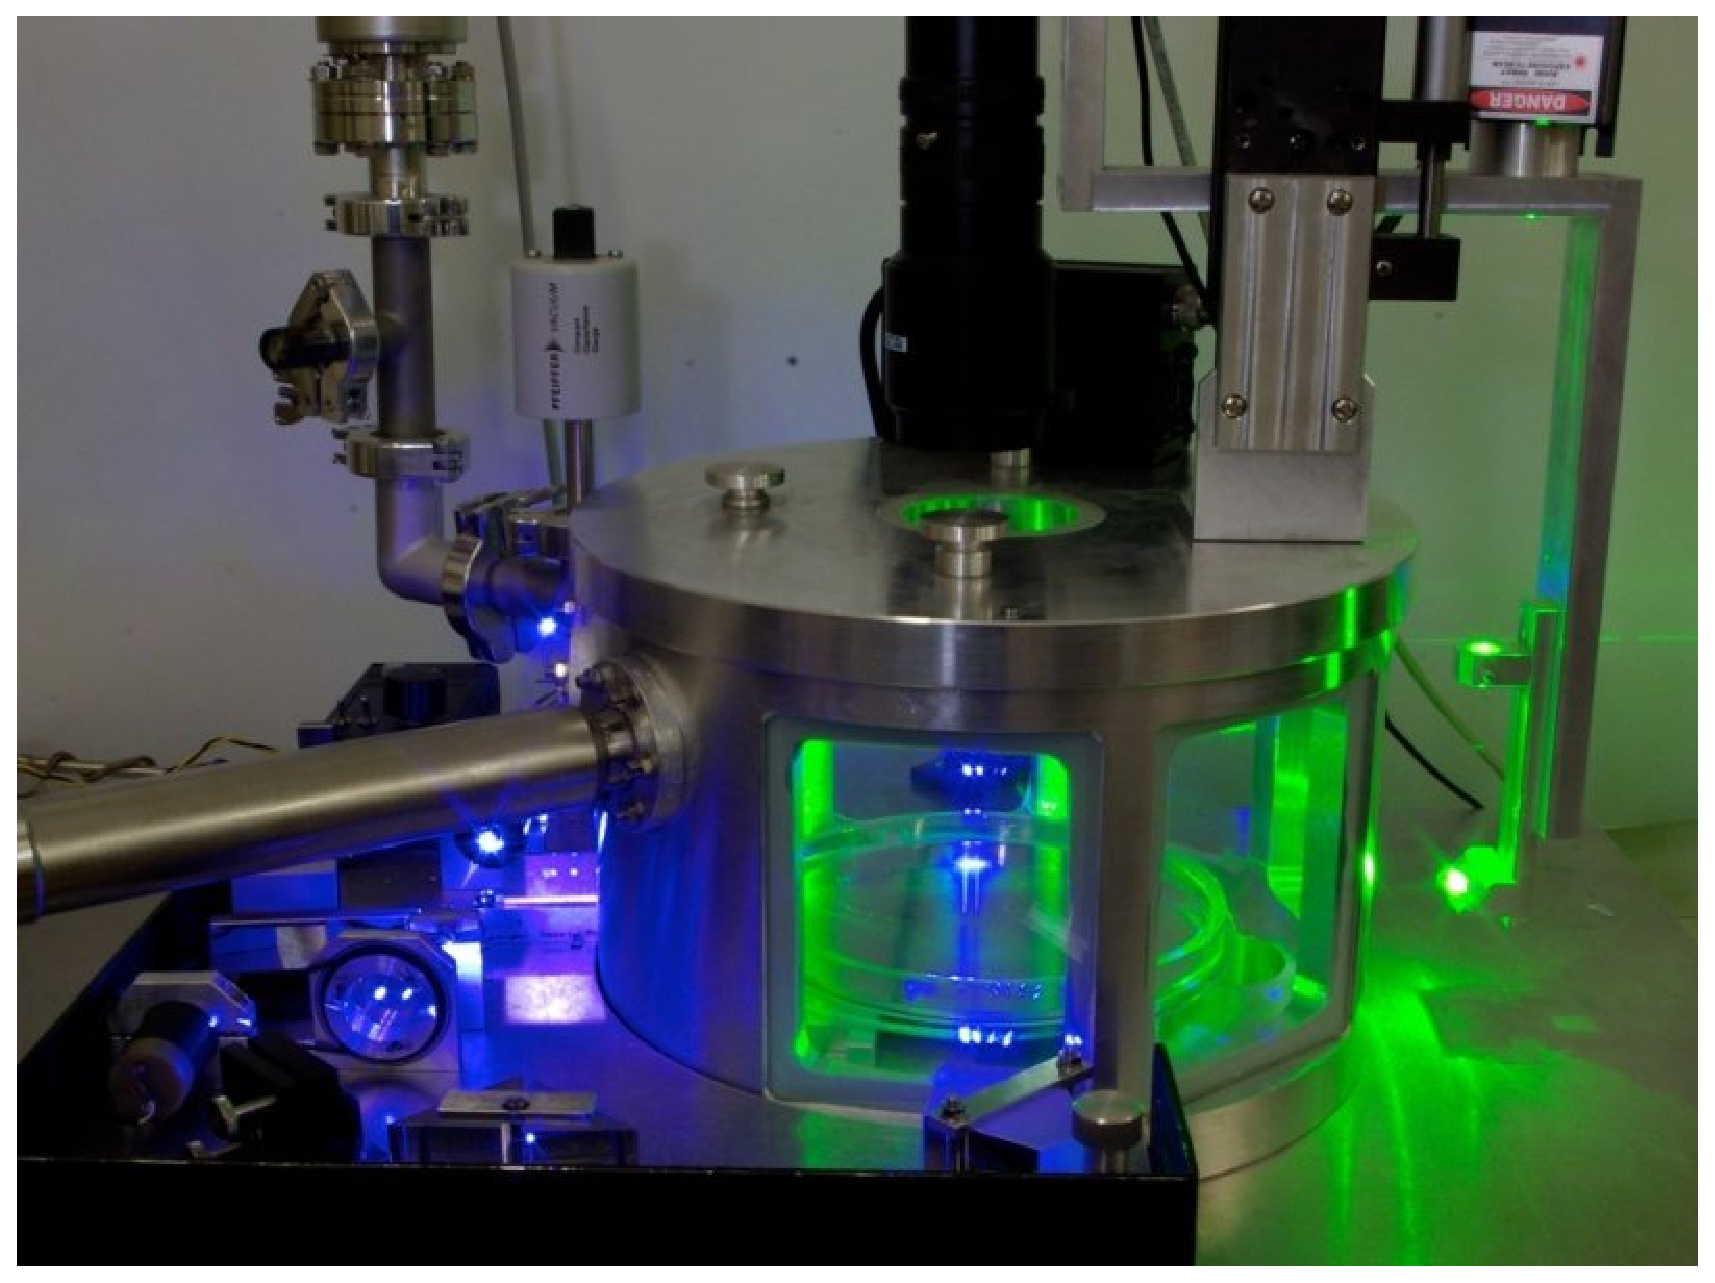
\includegraphics[width=0.9\columnwidth]{figures/eps/dusty2.eps}
		\caption{A konkrét kamra működése közben} 
		\label{fig:kamra}
	\end{figure}
	
%----------------------------------------------------------------------------
\section{A mérendő mennyiségek és a származtatott értékek}
%----------------------------------------------------------------------------
	A kísérlet előkészítése a következő lépésekből áll:
	\begin{enumerate*}
		\item Elővákum szivattyú bekapcsolása,
		\item Középvákuum szivattyú bekapcsolása,
		\item Argon palack megnyitása a megfelelő áramlás szintjére,
		\item RF gerjesztés bekapcsolása,
		\item Megvilágító lézer bekapcsolása,
		\item \label{it:por} Porrészecskék beszórása,
		\item Kamera bekapcsolása és a megjelenítő szoftver futtatása,
		\item Ha sok összetapadt porrészecske látható, illetve ha túl sok porrészecske látható, akkor
		az RF gerjesztés gyors ki-be kapcsolása után a \ref{it:por}.-től való folytatása a folyamatnak.
	\end{enumerate*}
	A \ref{fig:captures}. ábrán látható álló és forgó alsó elektródájú kísérlet során a
	porrészecskékről készült kép.
	
	\begin{figure}[!ht]
		\centering
		\subfloat[Álló elektróda esetén sok $\left(\sim 1500\right)$ részecske]{
			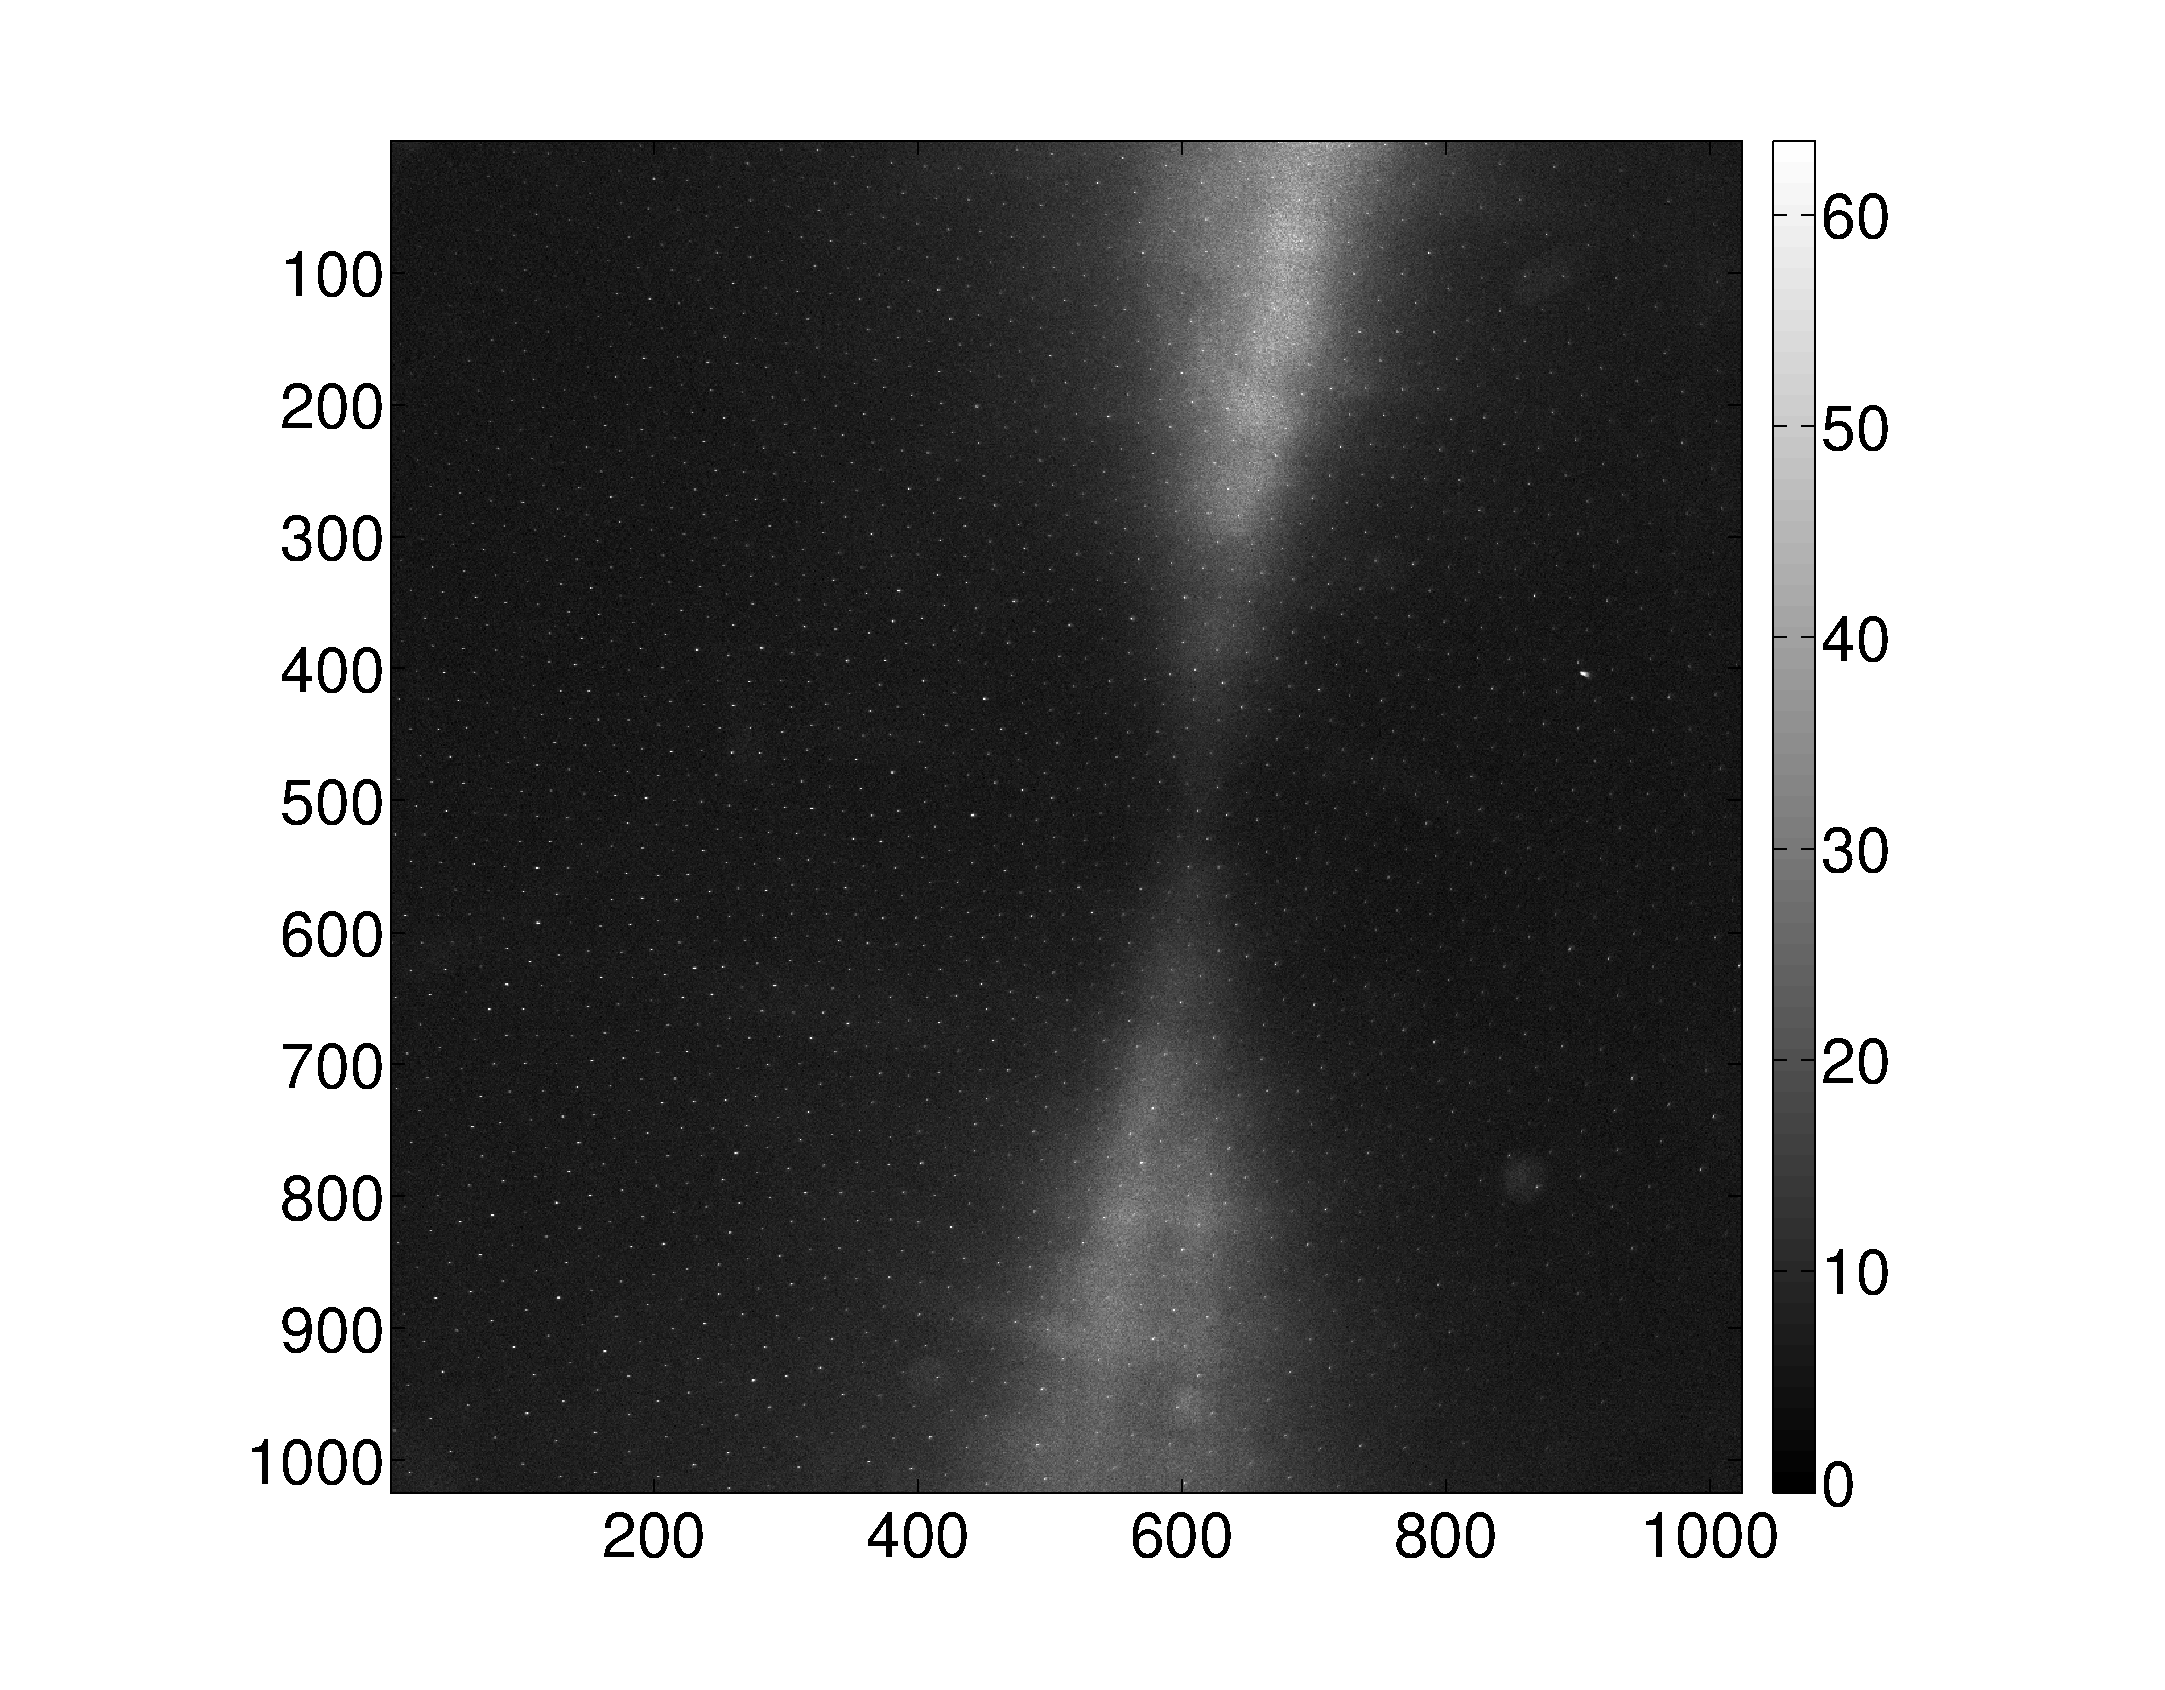
\includegraphics[width=0.95\columnwidth]{figures/eps/000047659380.eps}%
			\label{fig:allo}
		}
		\\
		\subfloat[Forgó elektróda esetén kevés $\left(\sim 100\right)$ részecske]{
			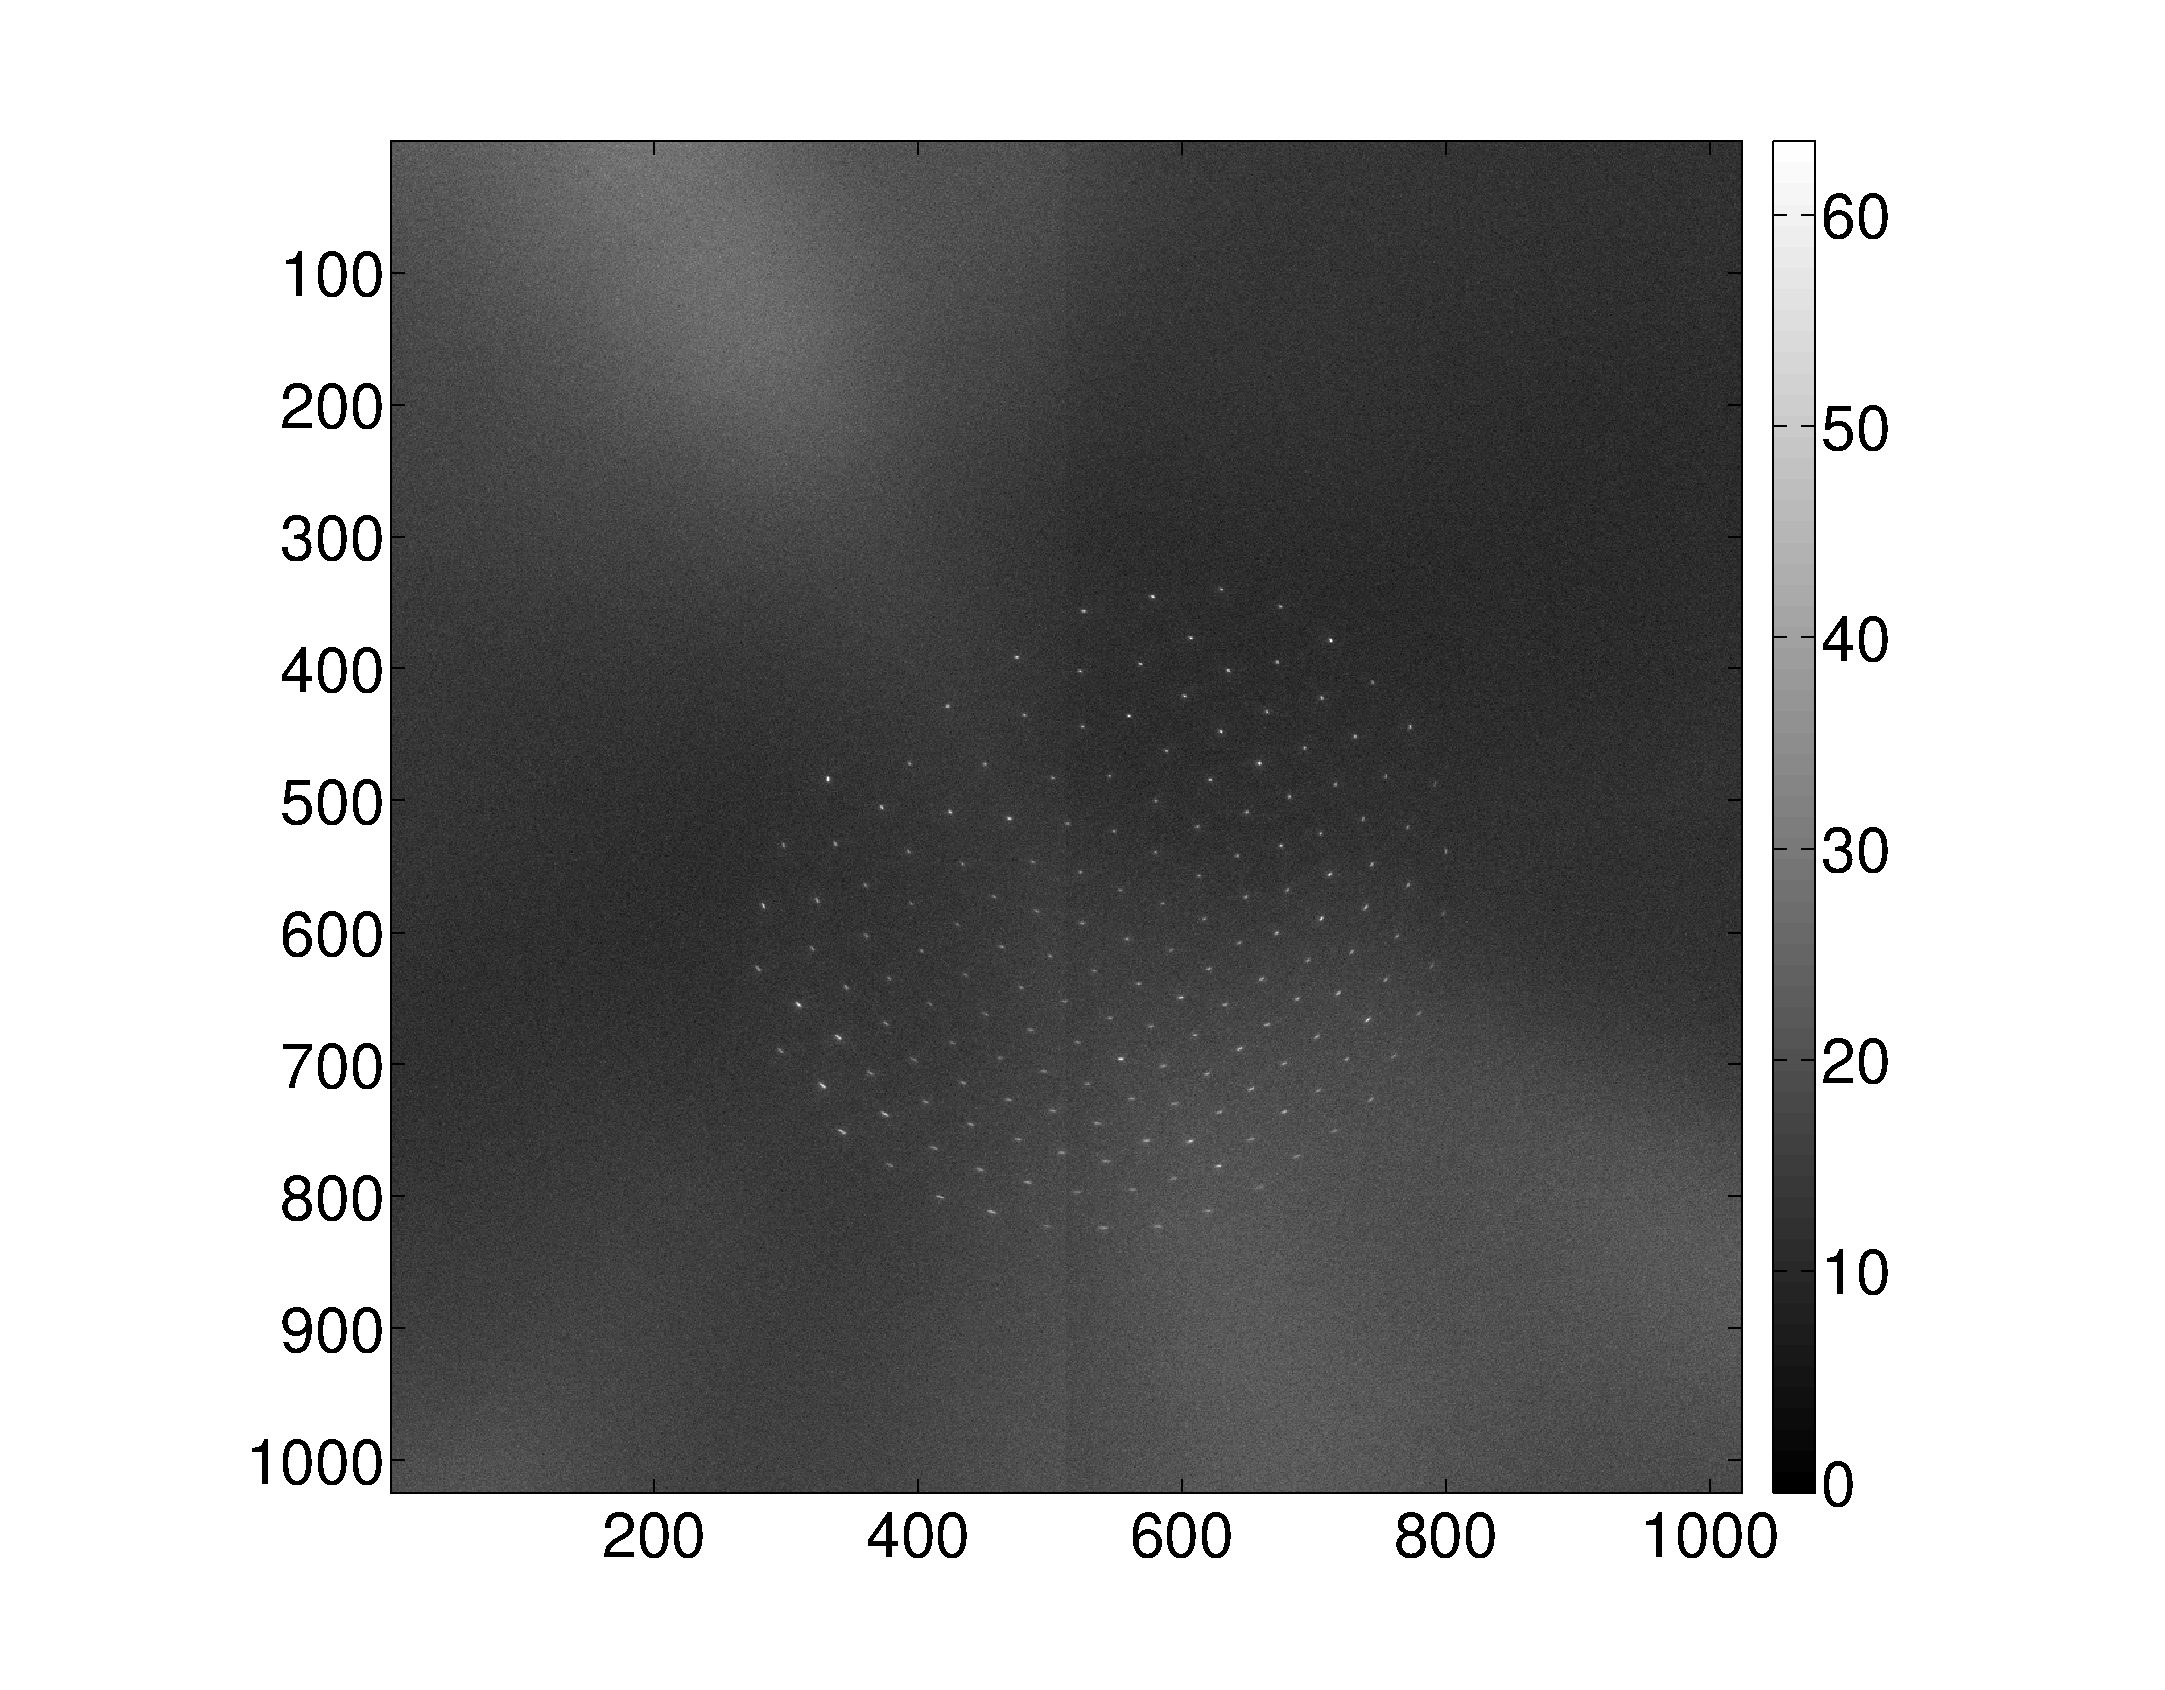
\includegraphics[width=0.95\columnwidth]{figures/eps/000000606627.eps}%
			\label{fig:forgo}
		}
		\caption{Két különböző kísérlet során készült fénykép.}
		\label{fig:captures}
	\end{figure}
	
	A fényképek alapján a részecskék pozíciójára és időbeli eloszlására vagyunk kíváncsiak.
	A kamera objektíve által leképezett kép a függőleges irányú pozíciót nem tartalmazza. Mivel jelen
	kísérletek során az ezirányú mozgása a részecskéknek nem számottevő, így az $x-y$ pozícióját jól
	lehet számítani a kép alapján. Nagy pontosság esetén szükséges a képek előzetes feldolgozása a
	perspektivikus torzítás kiküszöbölése végett. Természetesen ez lehetséges a pozíciók számítása után
	is, aminek a számításigénye kissebb is.




%----------------------------------------------------------------------------
\chapter{A részecskék detektálása}
%----------------------------------------------------------------------------

\section{Detektálási módszerek}
	A korábban látható \ref{fig:captures}. ábrán látható ábrákhoz hasonló képekről kell a részecskéket felismerni és
	azoknak a koordinátáit exportálni.
	Erre több lehetőség adódik, amit a \cite{Feng2007} részletez.
	A detektáló módszereket a számítás igényeiknek növekvő sorrendjében mutatom be.
\subsection{Küszöb módszer}
	Legkézenfekvőbb módszer, hogy a kép pixeleinek világosságát összehasonlítjuk egy küszöb értékkel
	és ha az nagyobb ennél, akkor ezeket megjelöljük, mivel ott részecskét feltételezünk. 
	A módszer egyenletes háttér-világosság esetén jól működik és extra gyorsan számítható.
\subsection{Küszöb módszer szűréssel}
	A háttér világossága a \ref{fig:allo}. ábrán jól láthatóan nem egyenletes.
	A korábban említett egyszerű küszöb módszer itt nem alkalmazható, mivel a világos és sötét
	területek más és más küszöbértéket kívánnának meg.
	A megoldása erre, mint megannyi villamosmérnöki mérési feladatra, hogy a jel helyett a
	differenciális jelet mérjük/számítjuk. Jelen esetben ez azt jelenti, hogy először előállítjuk a
	részecske nélküli háttérképét, majd a méréssel kapott képből kivonva ezt a differenciális képet megkapjuk.
	A differenciális képen a részecskéket a korábban említett küszöb módszerrel lehet detektálni a
	részecskéket.
	
	Ehhez csupán a mérési képből kell szűréssel származtatni a háttérképet azaz eliminálni a részecskéket.
	A \cite{Feng2007,Oxtoby2010} cikkekben és általában is erre véges Gauss szűrőt használnak, ami egy
	lineáris véges impulzusválaszú (FIR) aluláteresztő szűrő.
	A szűrés egy adott pixel környezetének súlyozott átlagolását jelenti.
	A súlyozás során szoroznunk kell, ami a bináris megvalósítás végett jóval lassabban történik, mint az
	összeadás avagy az összehasonlítás.
	
	Mivel a részecskék mérete a képen véges és kis szórású, így a korábban
	említett FIR Gauss szűrő aránylag jól tudja a részecskéket eliminálni.
	Viszont a mérési képek $100\ \mathrm{FPS}$ sebességgel és $1024\times1024$ mérettel érkeznek be.
	Ez $100\ \mathrm{MByte/s}$ adatfolyamot jelent. Ahhoz, hogy ezt közel real-time feltudjuk dolgozni
	a Gauss szűrés nem járható út. Hatékonyabb szűrőre van szükségünk! A megoldást a medián szűrőben látom,
	ami egy nemlineáris, de véges ``impulzusválaszú'' szűrő.
	A szűrő az adott pixel környezetének mediánjának számítását jelenti.
	A nemlinearitás jelen esetben nem okoz gondot, mivel csak detektálásra használjuk (a pozíció
	kinyerése az eredeti kép alapján készül, de ez később részletezve lesz.)
	
	A Gauss szűrő $N = n\times n$ környezet (ablak) esetén $N^2$ szorzást és $N^2-1$ összeadást jelent. Míg
	a medián szűrő $N = n\times n$ ablak esetén: bubborék rendezés során $O(N^2)$, javított bubborék
	rendezés során $O(N^2 / 2)$, quicksort esetén $O(N\log N)$ illetve kiválasztásos rendezés esetén $O(N)$ összehasonlítást és
	cserét. Az összehasonlítás és a csere nagyságrendekkel gyorsabban végrehajtható, mint a szorzás és
	összeadás. A kedvező lépésszám és helybeli rendezés lehetősége végett a kiválasztásos rendezést választottam.
	
\subsection{Adaptív küszöb módszer szűréssel}
	Látható a \ref{fig:allo}. ábrán, hogy a sötétebb háttér kiterjedése nagyobb, ennek megfelelően az
	kamera expozíció szabályozója ezekre a területekre állítja be az expozíciót.
	Így a sötét területek részletesebbek, míg a világos területek részletszegények (túlexponáltak) lesznek.
	Számunkra ez azt jelenti, hogy a sötétebb területeken jobban megbízhatunk a részecskék kiugró
	értékében, míg a világosabb területeknél nem.
	Ezt a döntési küszöb értékének adaptációját jelenti a háttér világosságához.
	Az adaptív küszöböt a következő kifejezéssel határoztam meg:
	\begin{multline}
		\label{eq:treshold}
		K = \E{P-\mhat{M}P}+\\
		  + \delta \cdot \STD{P - \mhat{M}P} \cdot 
		\left[ 1+ a \left(
			\frac{\mhat{M}P}{\max\left\{\mhat{M}P\right\} - \min\left\{\mhat{M}P\right\}}
			\right)^b
		\right]
	\end{multline}
	ahol $P$ az eredeti kép, $\mhat{M} P$ a medián szűrt kép, $\E{\ }, \STD{\ }$ az
	átlag és a szórás számításának függvénye és az $a, b, \delta$ három alakparaméter.
	\footnote{Az adaptív döntést a mérési kép előzetes feldolgozásával is elérhettük volna,
	ha a Photoshop-ból ismert Curves tool-hoz hasonlóval módosítottunk volna rajta. (A tool a képre egy nemlineáris
	függvénnyel hattat.)}
	
	A \ref{fig:alg}. ábrán látható a detektálási algoritmus működése közben.
	A \ref{fig:alg1}. ábrán a mérési kép ($P$) látható kitöltött görbével, ami az \ref{fig:allo}. ábrán
	látható mérési kép $x=40$ sora.
	Piros görbével látható a medián szűrt jelet ($\mhat{M}P$), amin jól érzékelhető a hirtelen
	változások eliminációja.
	A következő \ref{fig:alg2}. ábrán az eredeti és a szűrt különbsége azaz a differenciális kép
	($P - \mhat{M}P$) látható a kék görbével. A zöld görbe a \eqref{treshold} szerinti
	döntési köszöb.
	Az utolsó \ref{fig:alg3}. ábrán a detektált részecskék figyelhetőek meg.
	
	\begin{figure}[!h]
		\centering
		\subfloat[Eredeti (kitöltött) és a medián szűrt (folytonos) jel]{
			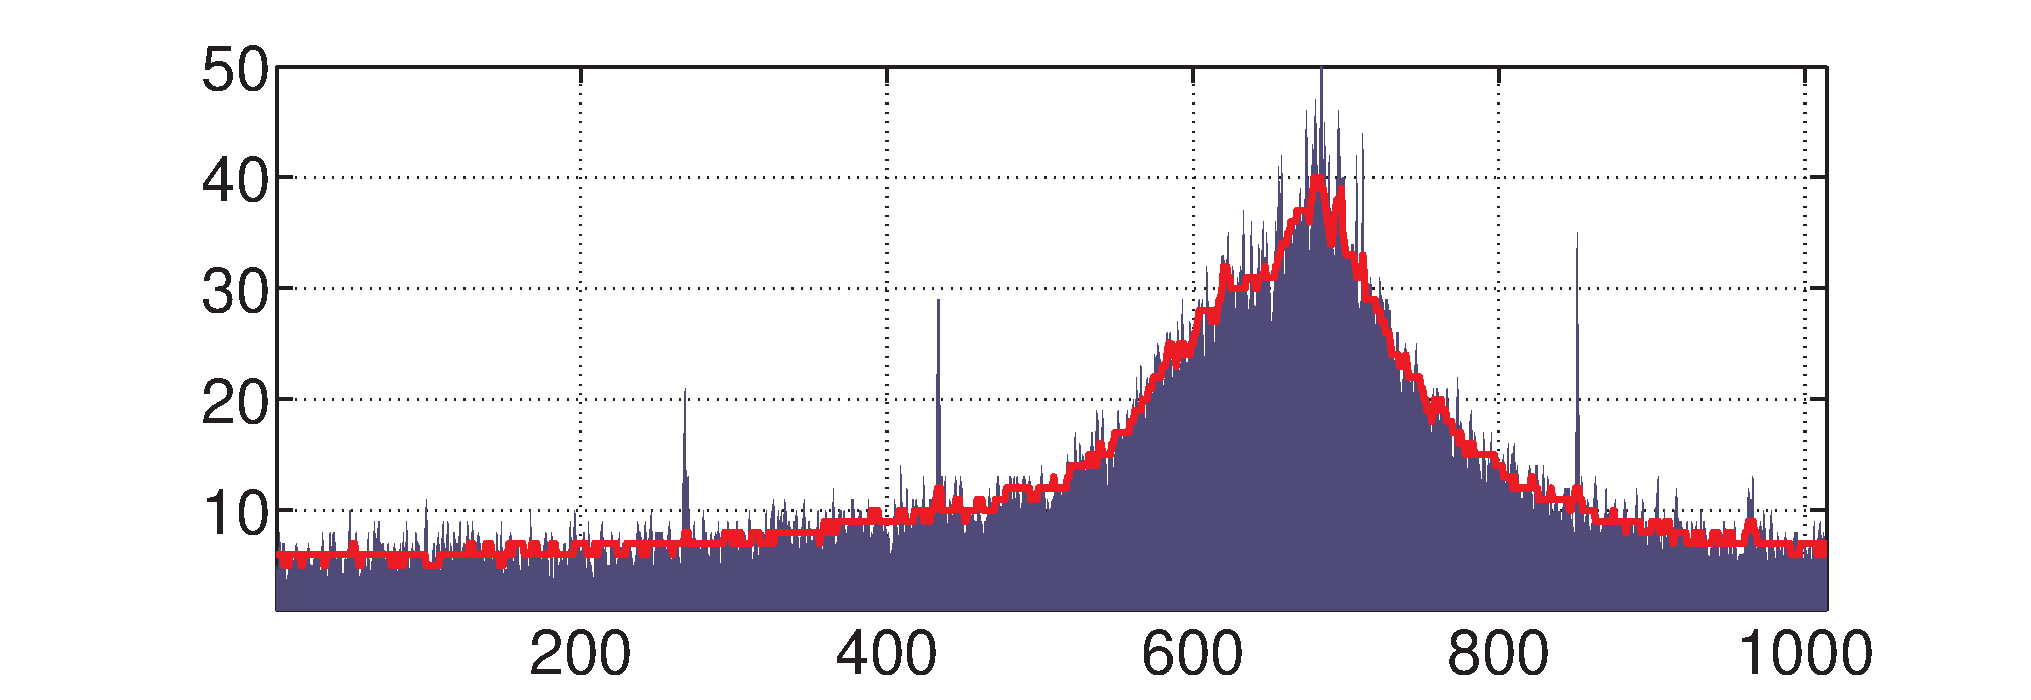
\includegraphics[width=0.95\columnwidth]{figures/eps/algoritmus1.eps}%
			\label{fig:alg1}
		}
		\\
		\subfloat[A differenciális jel (kék) és a döntési küszöb (zöld)]{
			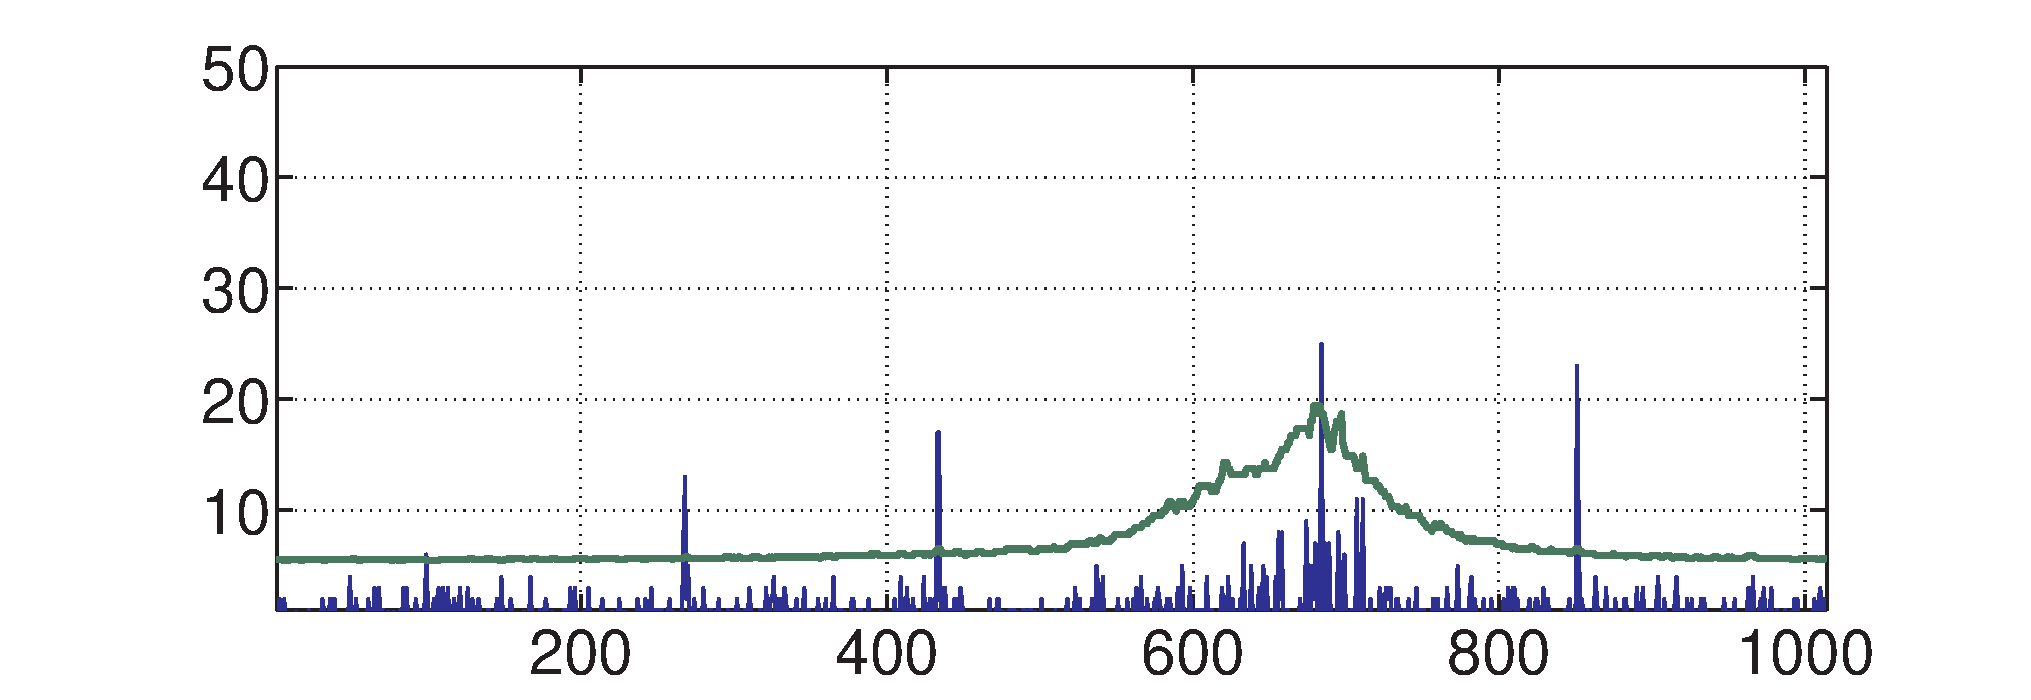
\includegraphics[width=0.95\columnwidth]{figures/eps/algoritmus2.eps}%
			\label{fig:alg2}
		}
		\\
		\subfloat[Detektált részecskék]{
			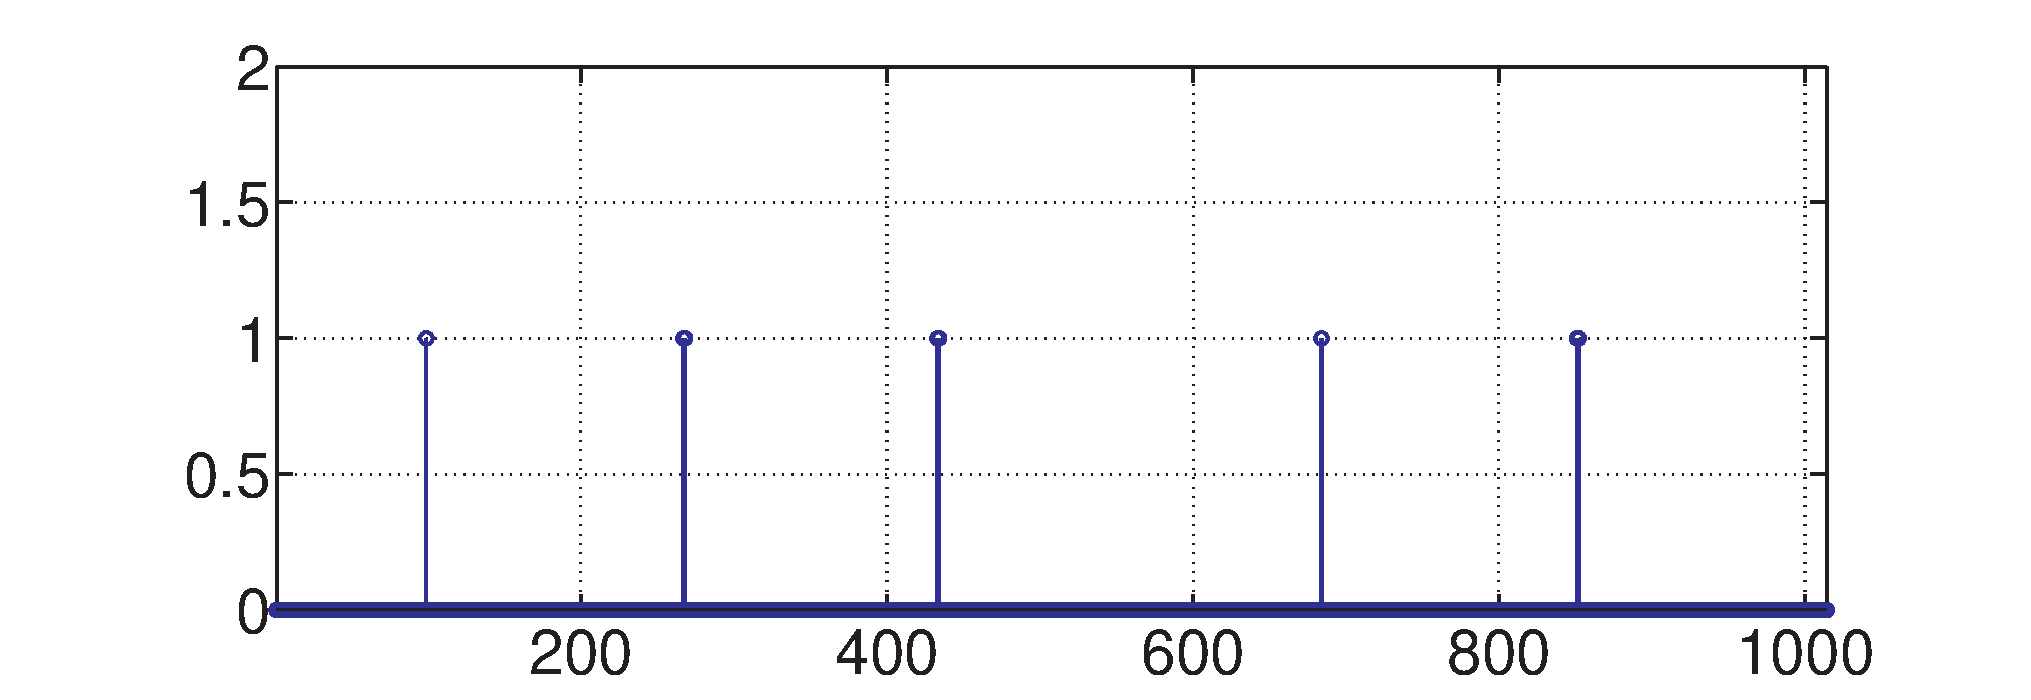
\includegraphics[width=0.95\columnwidth]{figures/eps/algoritmus3.eps}%
			\label{fig:alg3}
		}
		\caption[Adaptív küszöb bemutatása]{A medián szűrést alkalmazó adaptív küszöbbel részecskét
		detektáló algoritmus bemutatása az álló mérési kép (\ref{fig:allo}. ábra) $x=40$ során.}
		\label{fig:alg}
	\end{figure}
	
\section{A részecskék pozíciójának számítása}
	Kis felbontású kamera illetve nagyon kis porrészecskék esetén előállhat, hogy a részecskék csupán egy
	pixelnyi területet foglalnak el a képen. Detektálás szempontjából ez kedvező viszont a pozíciómérés
	szempontjából nem, mivel ilyenkor a felbontásunk 1 pixelnyi. Ezen javítani a dithereléssel a
	következőképpen lehet: picit elállítjuk az élességet úgy, hogy egy részecske több pixel nagyságú
	``maszat'' legyen, majd a korábban részletezett detektálást elvégezzük.
	
	Ennek hatására egy részecske több pixelnyi felületet fog elfoglalni és a detektáló algiritmus is
	több pixelt fog megjelölni. A pozíció megtalálásához csoportosítani kell a megjelölt pixeleket.
	Az egy részecskéhez tartozó pixel-csoportot egy téglalap fogja határolni, amit region of
	interest-el (ROI) szokás illetni. Azonban a részecske detektálása után amorf formájú megjelölt
	pixeleink lesznek. Ezeket a könnyebb csoportosítás végett kiterjesztem pár pixellel az így kapott
	pixeleket flood-fill algorimussal egybefüggővé teszem és ennek eredményeképp megkapom a ROI határoló
	koordiánáit, amit a következő két módszer felhasznál a részecske pozíciójának számítása során.
	\subsection*{Maximum keresés}
	Legegyszerűbb eset, ha a ROI-n belül az eredeti pixelek közül a legvilágosabbat veszem a
	részecske pozíciójaként.
	\subsection*{Szubpixel felbontás momentum módszerrel}
	Szofisztikáltabb, ha a ROI-n belül az eredeti pixelek világosságát, mint tömegpont tömegének veszem
	és a ROI-által határolt test súlypontját megkeresem. A módszerre kritikusan hat az előbb említett
	kiterjesztés mértéke. Ha túl nagy a kiterjesztés, akkor azzal hibát viszek be pozicíó mérésébe,
	míg ha túl kicsi akkor meg egy részecskének akár két képe/pozíciója keletkezhet. Továbbá nem érünk el nagyobb pontosságot a
	maximumkereséshez képest.
	
	\noindent Az algoritmus hatékonyságát különböző $\delta$ érték mellett a következő \figref{roi}
	ábrán látható.
	
	\begin{figure}[!ht]
		\centering
		\subfloat[$\delta = 10$]{
			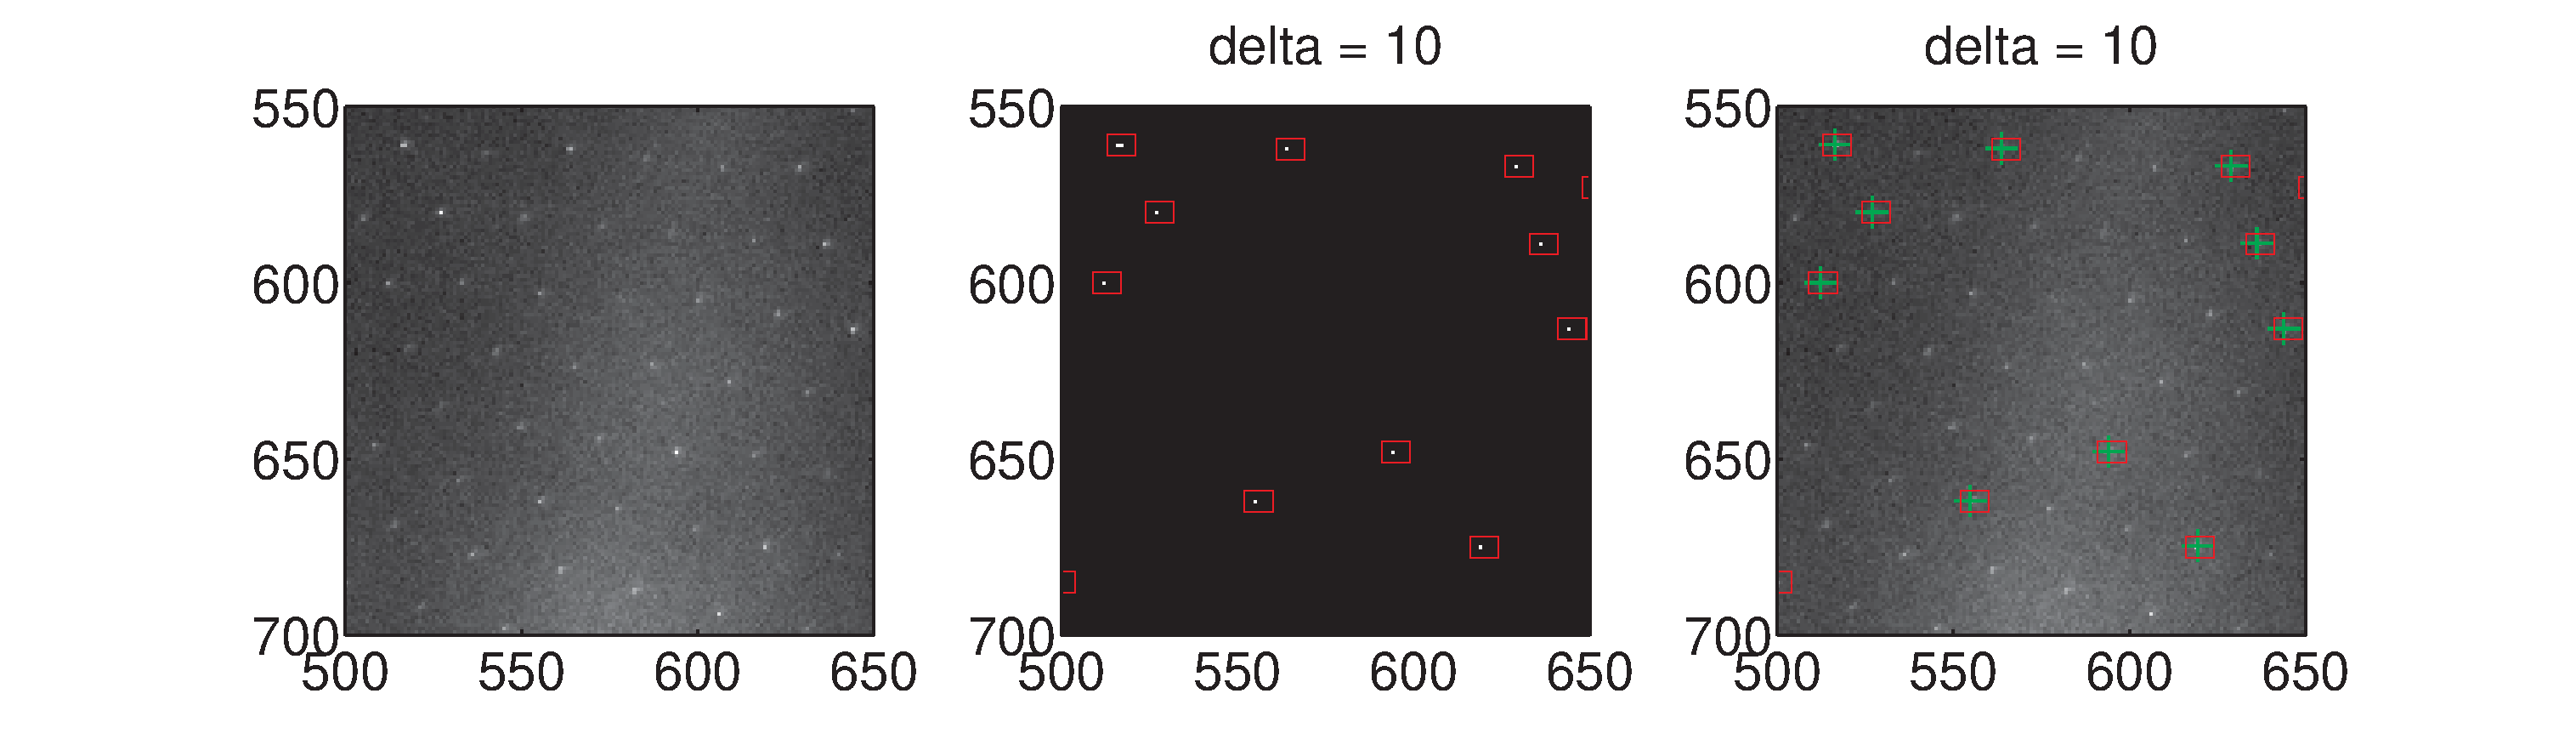
\includegraphics[width=1\columnwidth]{figures/eps/delta10.eps}%
			\label{fig:delta4}
		}
		\\
		\subfloat[$\delta = 2$]{
			\includegraphics[width=1\columnwidth]{figures/eps/delta2.eps}%
			\label{fig:alg3}
		}
		\\
		\subfloat[Optimális $\delta = 3.5$]{
			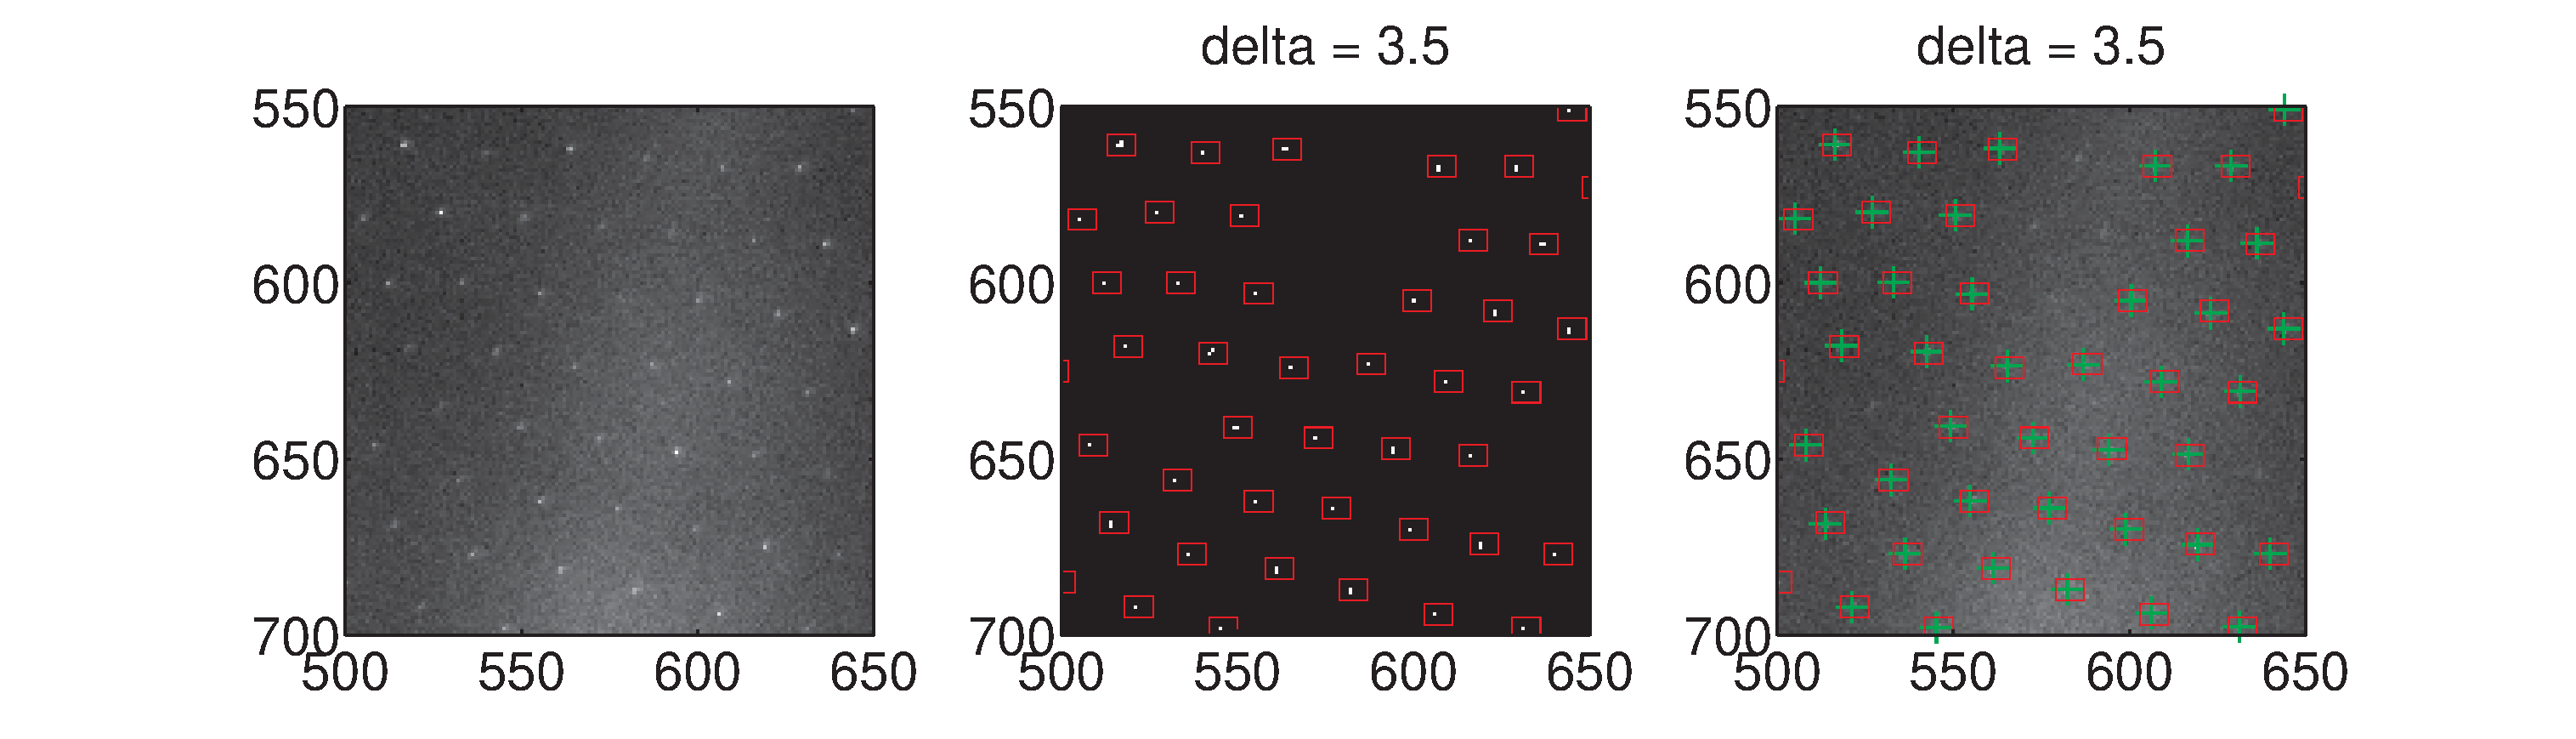
\includegraphics[width=1\columnwidth]{figures/eps/deltaopt.eps}%
			\label{fig:deltaopt}
		}
		\caption[Pozíciómérés momentum módszerrel]{Az adaptív küszöb módszerrel detektált részecskék
		momentum módszerrel számított pozíciója. \textbf{Bal oszlopban} az eredeti mérési kép egy részlete, \textbf{középső oszlopban} a
		detektálás eredménye és a ROI, az \textbf{utolsó oszlopban} az eredeti mérési képen a ROI és a detektált
		részecske pozícióját jelző kereszt.}
		\label{fig:roi}
	\end{figure}
	
	\noindent
	\begin{center}
	Az algoritmus jól párhuzamosítható, ami a nagyteljesítményű multiprocesszoros
	környezetben kedvező futási időt eredményezhet. A párhuzamos program létrehozásának segítségére az 
	OpenCL keretrendszert választottam, aminek a bemutatása következik.
	\end{center}






%----------------------------------------------------------------------------
\chapter{A multiprocesszoros OpenCL környezet} \label{sec:opencl}
%----------------------------------------------------------------------------

\section{OpenCL architektúrája}
	Az Open Computing Language (OpenCL) keretrendszer \cite{opencl}
	általános modellt, magas szintű programozási interfészt és hardware
	absztrakciót nyújt a fejlesztőknek adat-, vagy feladat párhuzamos számítások gyorsítására különböző
	számítóegységen (CPU, GPU, FPGA, DSP, \ldots).
	A hardvergyártók implementálják az OpenCL szabványt, ami által saját platformot
	hoznak létre. Egy ilyen platformon belüli eszközök alatt főként GPU-kat, de
	CPU-kat és FPGA-t \ldots is értünk.
	OpenCL keretrendszerben történő programozás során két programot kell írnunk.
	Az egyik a kernel, ami az eszközön futtatott szálra fog leképeződni.
	A másik a gazda processzoron (host-on) futó host-program, ami elvégzi az I/O műveleteket,
	a probléma összeállítását, a memória allokálást, az argumentumok beállítását
	illetve a kernel meghívását az eszközön.
	A kernel futása végeztével a host-program kiolvassa az eszközből
	a kívánt eredményt.
	
	\begin{figure}[!ht]
		\centering
		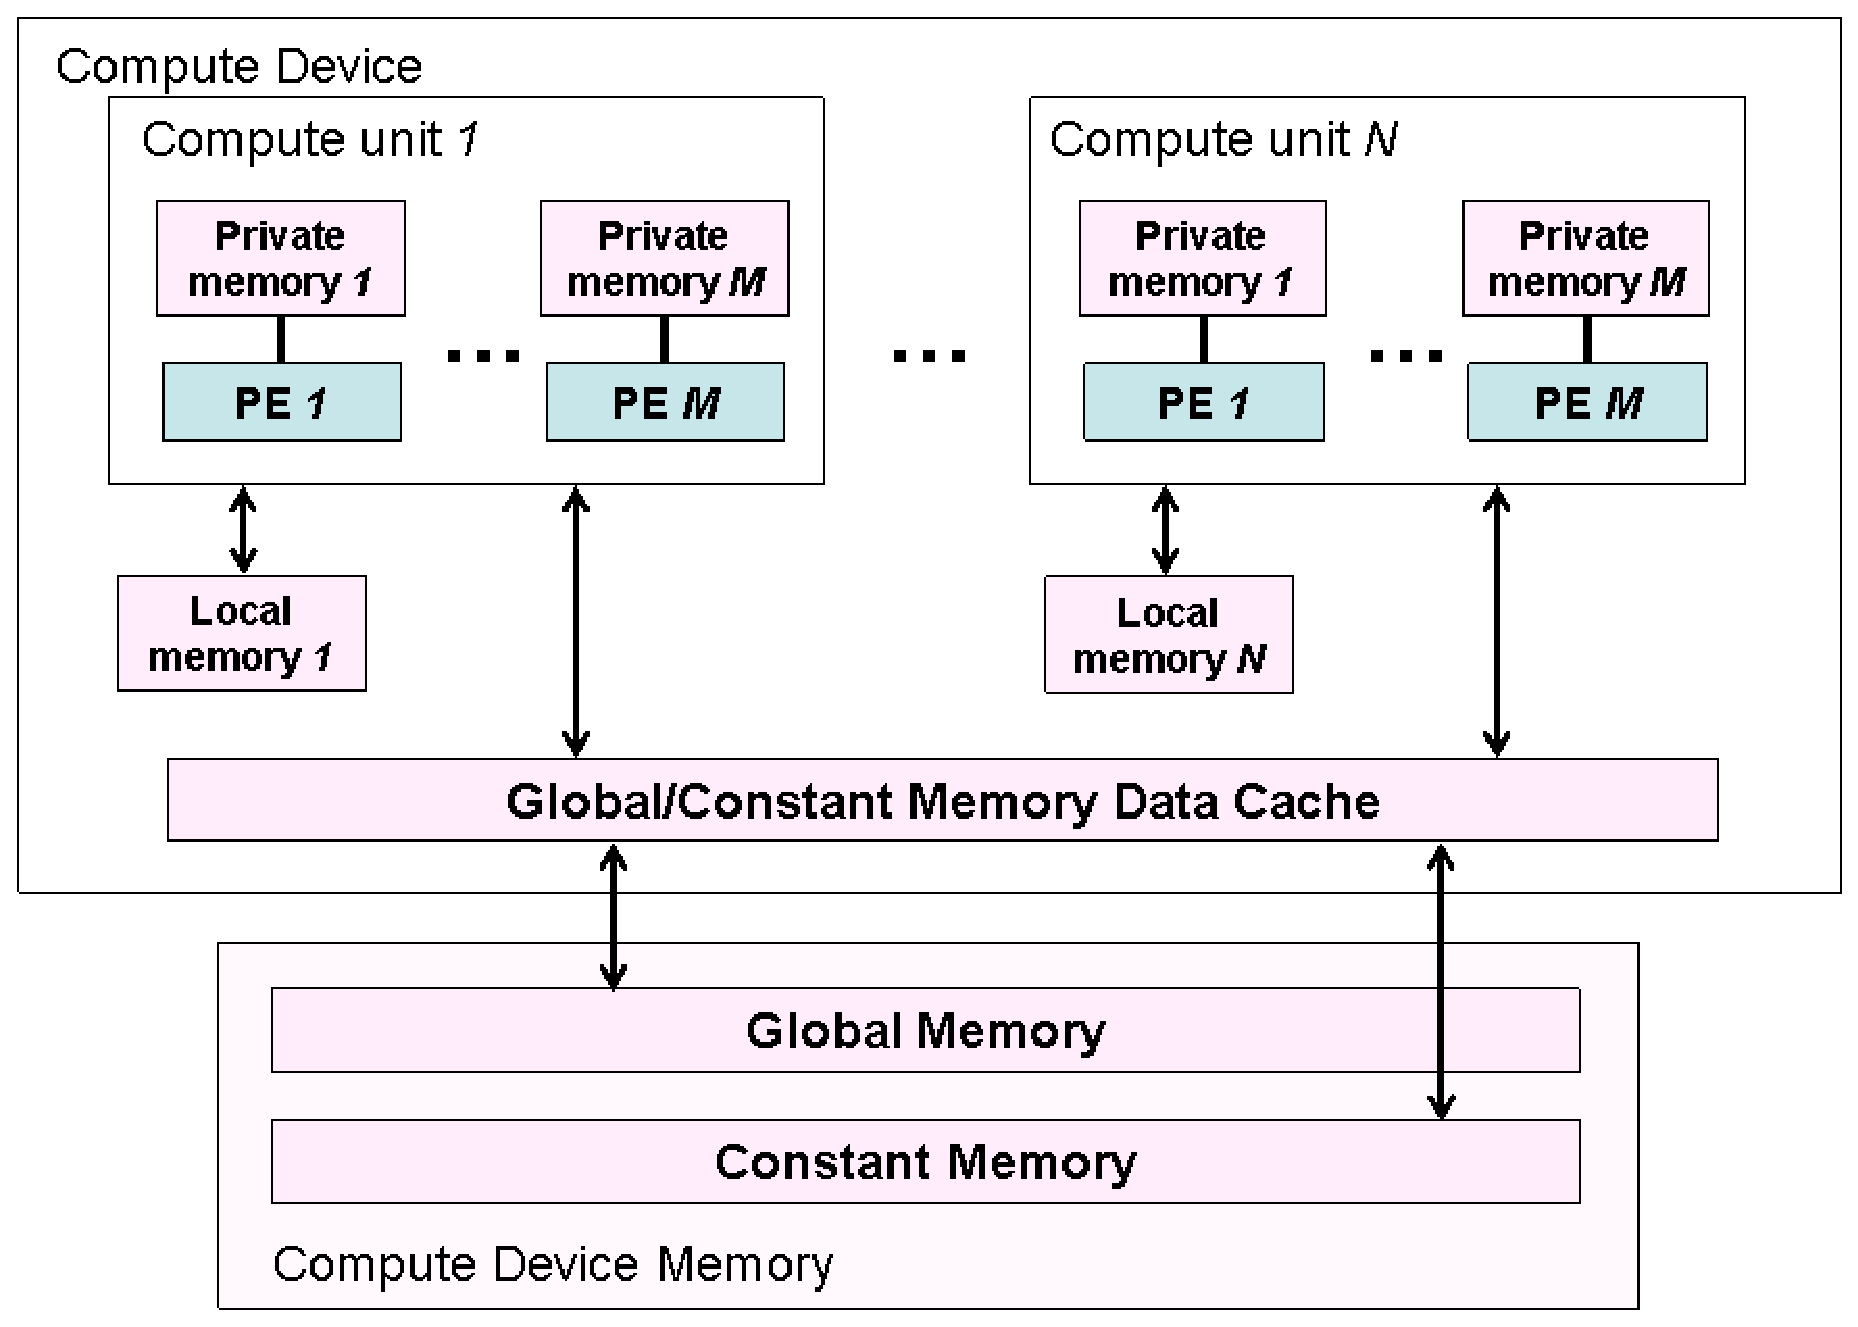
\includegraphics[width=0.6\columnwidth]{figures/eps/device.eps}
		\caption[OpenCL device architektúra]{OpenCL device architektúra (forrás: \cite{opencl})} 
		\label{fig:device} 
	\end{figure}
	Az eszközök multiprocesszoros architektúrával és ezek kiszolgálására képes
	memória architektúrával rendelkeznek, amit a \ref{fig:device} ábra vázol.
	Egy eszköz több compute unit-ot (processzor-magot) tartalmaz.
	Az OpenCL négy memória szintet különböztet meg, amikre a
	következőképpen hivatkozik:
	\begin{itemize}
		\item \emph{Regiszterek:} Private memory,
		\item \emph{Chipen belüli memória (cache):} Local memory,
		\item \emph{Chipen kívüli memória:} Global memory és Constant Memory.
	\end{itemize}
	A regiszterek és lokális memória kis méretűnek és gyors elérésűnek mondható, míg
	a globális memória nagynak, de lassú elérésűnek.
	A memóriákra megkötésként szolgál, hogy ki allokálhat, írhat és olvashat
	belőle. A \ref{table:mem}. táblázatban látható ezen jogosultságok.
	\begin{table}[!h]
	%\renewcommand{\arraystretch}{1.3}
	% if using array.sty, it might be a good idea to tweak the value of
	% \extrarowheight as needed to properly center the text within the cells
	\centering
	% Some packages, such as MDW tools, offer better commands for making tables
	% than the plain LaTeX2e tabular which is used here.
	\begin{tabular}{l|l|l|l|l}
			 & Global memory & Constant mem. & Local mem. & Private mem.\\ \hline
		Host & Dinamikusan R/W & Din. R/W & Din. R/W & \\
		Kernel & R/W & Statikusan R & Satik. R/W & Statik. R/W\\
		Sebesség & Lassú & Gyors & Gyors & Regiszter\\
		Méret & $1$ Gbyte $<$ & $\sim64$ Kbyte& $\sim16$ Kbyte & $<1$ Kbyte
	\end{tabular}
	
	\caption{OpenCL memória szintek}
	\label{table:mem}
	\end{table}
	
	Ahhoz, hogy a rendszerben rejlő teljesítményt kihozzuk három fontos kérdést
	kell a szimulátor magjának implementálásakor megválaszolnunk:
	\begin{itemize}
		\item \emph{Mennyit?} Tisztában kell lennünk az aktuális
		memória fogyasztással és a szükséges memóriamérettel.
		\item \emph{Honnan-hova?} Fontos, hogy a lehető legközelebb legyen az adat
		a processzor-maghoz.
		\item \emph{Mikor?} Mivel a memória művelet alatt a futtatott kernel nem
		dolgozik, így átadja a helyét egy másiknak. (Ez Direct Memory Access (DMA)
		blokk létezése alatt igaz). Ennek a megfelelő szinkronizációjával nagyobb
		kihasználtság érhető el (load balance).
	\end{itemize}
	
	
\section{OpenCL programozási modell}
	
	A programozási modell középpontjában a kontextus áll, ami az OpenCL
	osztálydiagramján (\ref{fig:class}. ábra) figyelhető meg.
	A futtatáshoz szükséges, hogy a kontextushoz platformot, majd azon belül
	eszközt, az eszközhöz programot (kernelt) és memóriát rendeljünk.
	\begin{figure}[!ht]
		\centering
		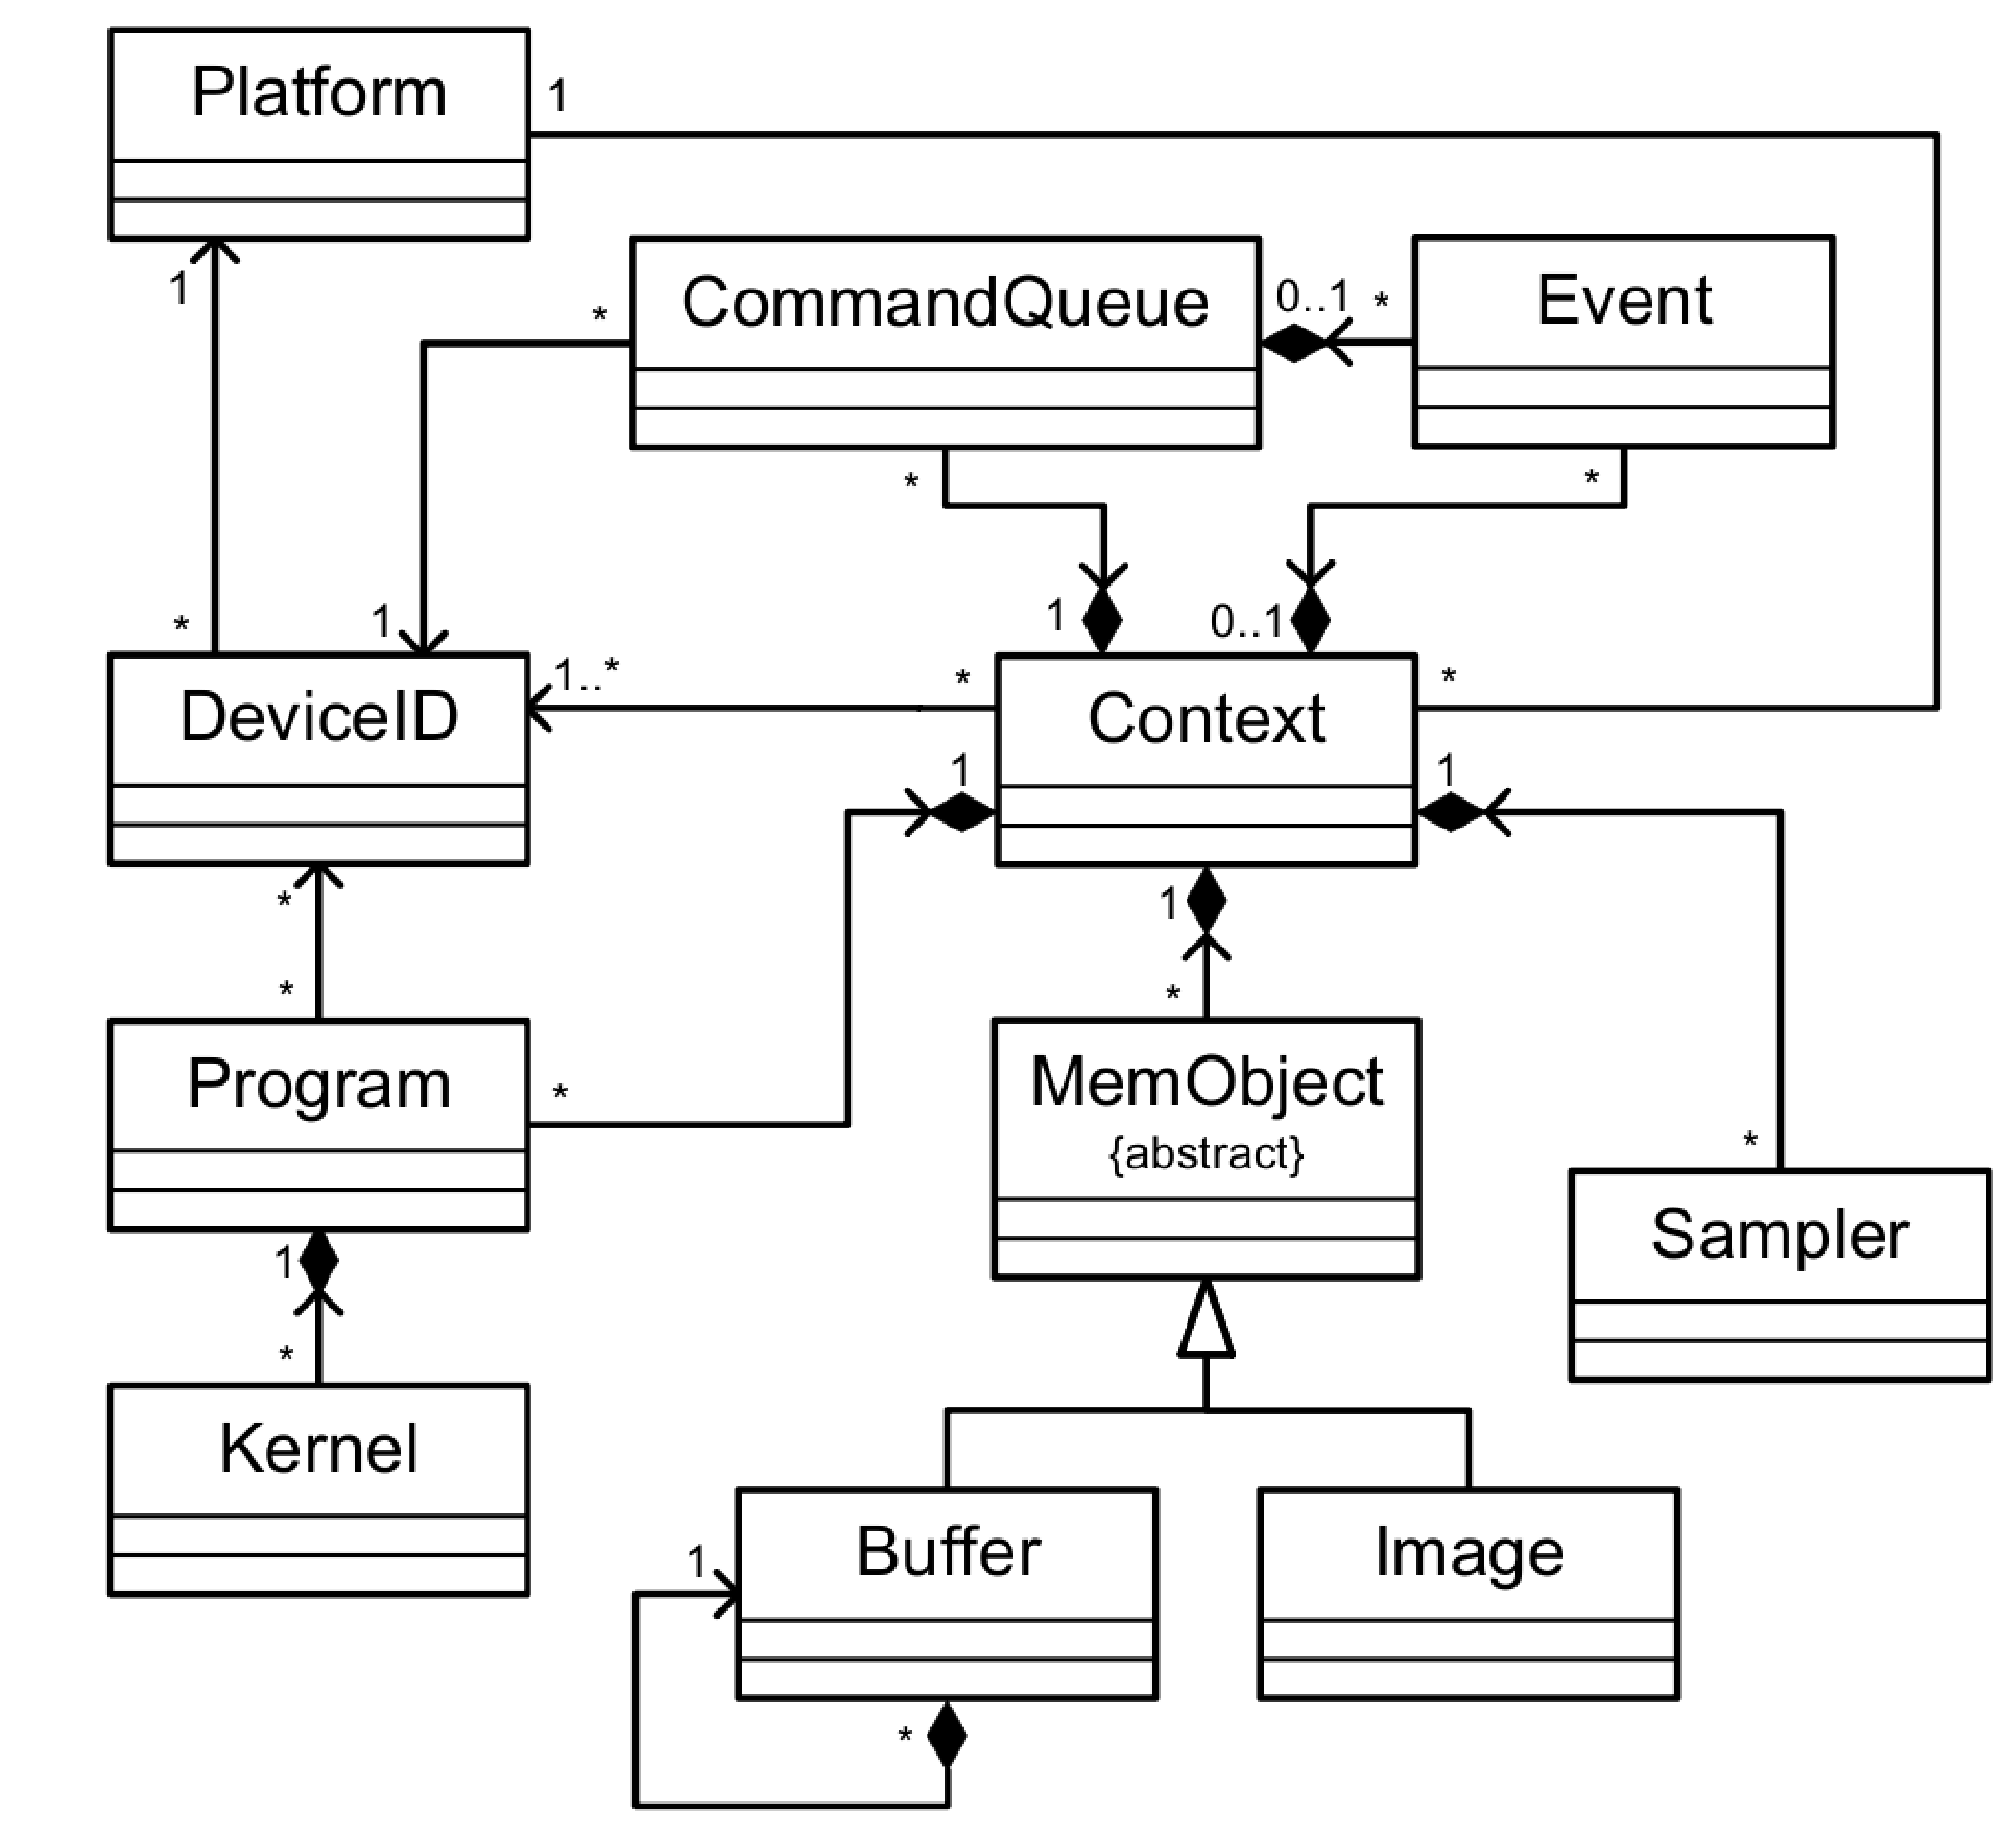
\includegraphics[width=0.6\columnwidth]{figures/eps/context.eps}
		\caption[OpenCL context osztálydiagrammja]{OpenCL context osztálydiagrammja (forrás: \cite{opencl})} 
		\label{fig:class} 
	\end{figure}
	Figyelembe kell vennünk azt a megkötést, hogy csak az egy platformon belüli
	eszközök programozhatóak heterogén módon. Például: Intel platform esetén
	lehetséges CPU-t, processzorkártyát és Intel-es GPU-t programozni.
	
	A programozással megoldandó problémát kétféleképpen lehetséges a feldolgozó
	egységekhez (work-item) avagy processzorokhoz rendelni:
	adat parallel módon vagy taszk parallel módon.
	
	Adat parallel módon (\ref{fig:data_parallel} ábra) a feldolgozandó adat egy
	részéhez rendelünk egy feldolgozó egységet. Fontos figyelembe venni az eszköz korlátos
	számú feldolgozó egységének számát. Ha nem elég a 
        rendelkezésre álló feldolgozó egység, akkor a
	feladat megfelelő particionálásával lehetséges az aktuális
        konfiguráció erőforrásaihoz illeszkedni.
	
	Taszk parallel módot (\ref{fig:task_parallel} ábra) olyan esetben célszerű
	használna, ha a bemenet dinamikus mérete a futási időben
        rendkívül változik
	illetve a végrehajtandó feladat lazán függenek össze.
	
	\begin{figure*}[!ht]
		\centering
		\subfloat[Adat parallel]{
			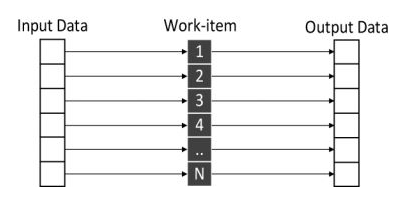
\includegraphics[width=0.45\columnwidth]{figures/eps/data.eps}%
			\label{fig:data_parallel}
		}
		\hfil
		\subfloat[Taszk parallel]{
			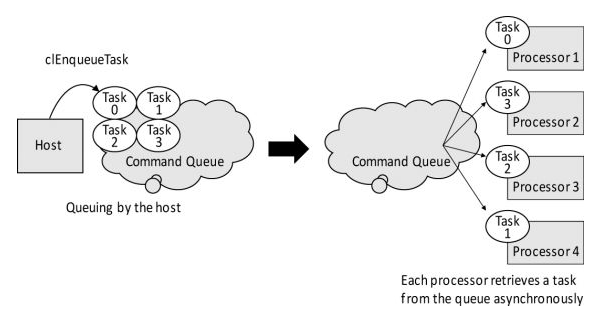
\includegraphics[width=0.45\columnwidth]{figures/eps/task.eps}%
			\label{fig:task_parallel}
		}
		\caption{Feladat hozzárendelése work-item-hez (processzorhoz)}
		\label{fig:parallel}
	\end{figure*}
	A processzor-magok megfelelő kihasználtságának elérése végett több ezer
	work-item virtuálisan osztozik rajta.
	Továbbá ezen work-item-eket work-group-okba rendezzük.
	
	A work-itemeket jelen pillanatban az OpenCL specifikációja
        \cite{opencl} szerint max. 3 dimenziós
	work-group-ba tudjuk rendezni. A következő \ref{fig:ndrange}. ábrán egy 2D-s példát láthatunk egy work-item indexének a globális
	és lokális megfelelőjére.
	
	\begin{figure}[!h]
		\centering
		\includegraphics[width=0.9\columnwidth]{figures/eps/ndrange.eps}
		\caption[2D-s work-item-ek work-group-ba rendezése és indexelése]{2D-s work-item-ek work-group-ba rendezése és indexelése
		(forrás: \cite{opencl})}
		\label{fig:ndrange} 
	\end{figure}

	A work-group-okba rendezés a lokális memória jogosultsága miatt érdekes.
	Konkrétan az egy work-group-ba tartozó összes work-item azonos lokális memórián
	osztozik.
	Ennek a következménye az, hogy adat parallel módú feldolgozás esetén
	az egymásra ható adatokhoz tartozó work-item-eket egy work groupba kell
	rendelnünk.
	Ha ez nem lehetséges, akkor a globális memóriához kell fordulnunk.
	A globális memória avagy a bank szervezésű külső (off-chip) memóriák
	hozzáférési ideje relatíve nagy így ezek használatát lehetőleg el kell kerülni
	és a programozónak kell ``cachelni" a lokális memóriába.
	
	Mivel a work-item-ek konkurensen hajtódnak végre, így az általuk közösen elérhető memóriákra
	(globális, lokális) nézve versenyhelyzetben vannak.
	Az OpenCL ezt a problémát a laza memóriamodell használatával oldja meg. Az alkalmazott
	szinkronizáció egy korlátot tesz a programban, amit csak akkor léphet át, ha az összes többi
	work-item az azonos work-group-ban ezt a korlátot már elérte. Erre a \texttt{barrier(FLAG)}
	függvényhívás szolgál. Fontos megjegyezni, hogy ez a szinkronizáció csak egy adott
	work-group-on belül történik, a work-group-ok közötti szinkronizációra nincs lehetőség. 
	
	\begin{center}
	Összefoglalva: nagy hangsúlyt kell a memóriaszervezésre fordítani, hogy a
	processzormagok megfelelően legyenek az adatokkal táplálva.
	\end{center}


\section{Futási környezet bemutatása}
	A következő eszközök teljesítményét vizsgálom:
	\begin{itemize}
		\item A laptopomban található \textbf{nVidia GTC 330m} notebook-videokártya,
		\item Asztali PC-ben található \textbf{Intel Xeon E5-1620} processzor,
 		\item Asztali PC-ben található \textbf{Intel Xeon Phi} co-processzor kártya \cite{phi,mic},
 		\item Asztali PC-ben található  \textbf{nVidia GTX 590} videokártya.
	\end{itemize}
	Ezen eszközök legjelentősebb paraméterei a \ref{table:envs} táblázat tartalmazza.
	
	\begin{table}[!h]
	%\renewcommand{\arraystretch}{1.3}
	% if using array.sty, it might be a good idea to tweak the value of
	% \extrarowheight  as needed to properly center the text within the cells
	\setlength{\extrarowheight}{8pt}
	\centering
	\footnotesize
	% Some packages, such as MDW tools, offer better commands for making tables
	% than the plain LaTeX2e tabular which is used here.
	\begin{tabular}{ l | r | r | r | r}
		 & nVidia GTX 330m & Xeon E5-1620 & Xeon PHI & nVidia GTX 590\\ \hline
		\texttt{MAX\_COMPUTE\_UNITS} & 6 & 8 & 224 & 16\\
		\texttt{MAX\_CLOCK\_FREQUENCY} & 1265 & 3000 & 1100 & 1225\\
		\texttt{MAX\_WORK\_GROUP\_SIZE} & 512 & 8192 & 8192 & 1024\\ \hline\hline
		\texttt{GLOBAL\_MEM\_SIZE} & 1\,Gbyte & 8\,Gbyte & 4.5\,Gbyte & 1.5\,Gbyte\\
		\texttt{MAX\_MEM\_ALLOC\_SIZE} & $\sim$ 0.25\,Gbyte & $\sim$ 8\,Gbyte & $\sim$ 1.5\,Gbyte & $\sim$ 0.4\,Gbyte\\
		\texttt{LOCAL\_MEM\_SIZE} & 16\,Kbyte & 32\,Kbyte* & 32\,Kbyte* & 48\,Kbyte\\
		\texttt{LOCAL\_MEM\_TYPE} & Local & Global & Global & Local\\
	\end{tabular}
	
	\caption{Használandó eszközök összehasonlítása}
	\label{table:envs}
	\end{table}
	
	Fontos kiemelni, hogy az Intel eszközeinek lokális memóriái (*) valójában a globális memóriából mappelt memóriaterület.
	
	Az összehasonlíthatóság végett a legkisebb memóriájú eszközre fogom a problémát skálázni. Tehát maximálisan 16\,Kbyte lokális
	memóriát fogok használni. A többi eszköz memóriája nagyobb, így a kód mindegyiken tud futni.
	


% ----------------------------------------------------------------------------
\chapter{A host program bemutatása}
% ----------------------------------------------------------------------------
	A 100~FPS-el érkező képeket az eszköz globális memóriájának méretét figyelembe véve dolgozom fel.
	Ha az eszköz memóriájába 100 képnél kevesebb fér be, akkor a másodperc fennmaradó képei eldobásra kerülnek. 
	A megjelenítésnek nem fontos szigorúan valós idejű működésűnek lennie (soft real-time), adott fokú késleltetés megengedhető 
	(határidő elmulasztása nem jár súlyos következménnyel). A program ciklikusan a következő felsorolásban olvasható lépéseket hajtja
	végre. A lépések a későbbi \ref{sec:parallel} részben ismertetettek végett párhuzamosan időben átlapolódva történnek. 
	\begin{enumerate*}
		\item Eszközön futtatandó kernelek inicializálása, argumentumainak beállítása,
		\item Kép fogadása (gyűjtése) a kamerától GigE interfészen keresztül (beolvasása a host-memóriába),
		\item Képek leküldése a host-memóriájából az eszköz globális memóriájába,
		\item Kernelek futtatása az eszközön:
		\begin{enumerate*}
			\item A másodperc első képének (medián) szűrése,
			\item Átlag és szórás számítása az eredeti és a szűrt kép különbségén (differenciális kép),
			\item Adaptív detektálási szint előállítása,
			\item Az első és a fennmaradó képeken detektálás.
		\end{enumerate*}
		\item Kernelek futása után az eredmény az eszköz globális memóriájából a host-memóriájába való
		visszatöltése,
		\item Posztprocesszálás és OpenGL megjelenítés.
	\end{enumerate*}
	A kernel megírása során a korábbi \ref{sec:opencl}. fejezetben említetteket figyelembe kell venni.
	Főként a véges lokális és globális memóriát és a work-itemek számát. A kernelek adat-parallel módon lett megírva.
	
\section{A host program párhuzamos felépítése} \label{sec:parallel}
	A korbábban megengedett késleltetésre és a real-time
        viselkedésre több tényező is rossz hatással van, ezek a következők:
	\begin{itemize}[noitemsep]
	  \item A kamera GigE interfészének jittere,
	  \item Operációs rendszer által futtatott egyéb folyamatok,
	  \item Feldolgozó (szűrő és detektáló) algoritmus futási idejének (ET = execution time) váltakozása. 
	\end{itemize}
	A kernelek közül a medián szűrő, ami elrontja a fix futási időt (Fix ET) és azt véletlenné teszi.
	A változó futási időről elmondható, hogy a bemeneti kép értékeitől függ. Pontosabban a medián szűrő ablakain belül található
	pixelek rendezettségétől. Hiszen minél rendezettebb, annál gyorsabban található meg a mediánját.
	A medián számításának worst case execeution time-ja (WCET), pontosabban WC lépésszáma ismert algoritmuselméletből, ami korlátos
	és megegyezik - a bemenet $N$ számossága esetén - a $O(\floor{N/2} \log N)$ értékkel.
	
	Adódik, hogy a host programot több konkurens szálra bontva kerüljön implementálásra az ismert Producer-Consumer
	\cite{EWD:EWD329pub} mintát alkalmazva. Ezzel elérhető, hogy a program feldolgozási sebessége ne a kép fogadásának és a kernel
	futási idejének összege legyen, hanem ezek közül a időben rövidebbig.
	Ez viszont szükségessé teszi, hogy az adatkapcsolatot a két szál között várakozási listával legyen biztosítva.
	Így a szálak egymásra várásának csökkentését lehet elérni.
	
	A szálak létrehozását és kezelését a \textit{Boost C++ Libraries} \cite{boost} keretrendszer
	megfelelő függvényhívásai oldják meg. A keretrendszer parancssori argumentumkezelést, szálkezelést, szemafort, várakozási
	listát és atomi működésű operátorokkal rendelkező változókat nyújt a programozó számára.
	A szálak közötti adatkapcsolást FIFO típusú (single producer - single consumer) várakozási listával oldom meg.
	
	A \texttt{Main} szálon kerül implementálásra a kamera képeinek fogadása és a várakozási sorba állítása\footnote{Természetesen a
	\texttt{main} szál a program felhasználó által történő
        futtatása által meghívott függvény, így az említettek előtt
        még inicializáció is történik. Ezt később részletezem. A szálra producer szálként kell tekintenünk a kamera képének fogadása és
	várakozási listába tétele végett.}.
	További consumer és egyben producer szálon a várakozási sorban található kép elővétele majd feldolgozására kerül sor az
	OpenCL kernel által, aminek eredménye a megjelenítő OpenGL bufferébe kerül letárolásra.
	Végül egy consumer szál a bufferben található eredmény OpenGL-es megjelenítést végzi.
	
	Az implementálandó szálak ``szekvencia diagramja'' a következő \ref{fig:host_seq} ábrán látható.
	Az ábra alapja UML szekvencia diagram, amit kiegészítettem az OpenCL kernel
	és az OpenGL callback függvényének futásával. Az ábrán három szál látható ezek a Main, CProducer, Consumer.
	A szálak részletes ismertetése a következő részben következnek.
	\newpage
	 
%\usepackage{graphics} is needed for \includegraphics
\begin{figure}[H]
\resizebox{\linewidth}{!}{\begin{sequencediagram}
	%\newthread{m}{\makebox[2cm]{Main}}
	\newthread{m}{Main}
	\newinst{prod}{\makebox[2cm]{CProducer}}
	\tikzstyle{inststyle}+=[left color = green, right color = red, rounded corners=3mm]
	\newinst[2]{ocl}{OpenCL}
	
	\tikzstyle{inststyle}+=[left color = white, right color = white, rounded corners=0mm]
	%\newthread{cons}{\makebox[2cm]{Consumer}}
	\newinst{cons}{Consumer}
	\tikzstyle{inststyle}+=[left color = blue, right color = blue, rounded corners=3mm]
	\newinst[1.5]{ogl}{OpenGL}
		\begin{call}{m}{start()}{cons}{join()}
		%\prelevel
			
		\begin{messcall}{cons}{start()}{ogl}
			\begin{call}{m}{start()}{prod}{join()}
			
			\begin{sdblock}{processingLoop}{}
				\mess{m}{input-queue}{prod}
				
				\begin{call}{prod}{enqueueKernel()}{ocl}{ReadBuffer()}
				\end{call}
				
				
				\begin{sdblock}{glutMainLoop()}{}
					\begin{call}{cons}{}{cons}{}
					\end{call}
				\end{sdblock}
				
				\mess{prod}{output-queue}{ogl}
				
				\begin{call}{ogl}{glutSwapBuffers()}{ogl}{}
				\end{call}
			\end{sdblock}
			
			\end{call}
			
		\end{messcall}
		
		\end{call}
	\end{sequencediagram}


}
	\caption{Host program ``szekvencia diagrammja''}
	\label{fig:host_seq}
\end{figure}

	
\section{Main (producer) szál}
	A programszál felhasználó által való indítással jön
        létre. Elsőként a program \texttt{main()} függvényét hajtja végre. A szál a
	parancssori argumentumok feldolgozását, az inicializálást és a kamera adatfolyamának fogadását és letárolását végzi.
	A paraméterek tárolására és konzisztenciájának megőrzésére definiáltam a következő osztályt:
\begin{lstlisting}[language=C++]	
class Params {
public:
	bool		only_global;	// csak globalis memoria hasznalata
	...
	uint		file_N;		// file merete def.: 1024
	uint		nh_N;		// median ablakanak merete !!! paratlan !!!
	uint		tail;		// a szures altal letrejovo pixelek a kep szelen 
	uint		Bfile_N;		// az igy kapott kep meret

	uint		pplN;		// kivant local meret

	uint		localN;		// work-group nagysage
	uint		globalN;		// osszes work-item szamossaga

	ulong	aSize;		// eszkoz global memoria max alloc. merete byte-ban
	ulong	lSize;		// eszkoz local memoria meret byte-ban

	ulong	mCuint;		// eszkoz max compute unit szama
};
\end{lstlisting}
	A paraméterek értelmezése a következő:
	\begin{description}[noitemsep]
	\item[only\_global] Csak globális memória használata vagy lokálisat is használjon. Egyes eszközök esetén a lokális memória a
	globális memóriába van mappelve, így használata csupán felesleges adatmozgatást jelentene $\texttt{only\_global} = 0$,
	\item[file\_N] A kép 2D-s mérete, $\texttt{file\_N} = 1024$,
	\item[nh\_N] A medián szűrő mozgó ablakának 2D-s mérete (páratlan szám) pl.: $\texttt{nh\_N} = 3,5,7,9$ (magasabb fokú szűrőt
	nem érdemes használni, mivel nagy nemlinearitással rendelkezne),
	\item[tail] a szűrés által létrejövő pixelek a kép szélén, azaz \texttt{tail = (nh\_N -1) / 2},
	\item[Bfile\_N] az így kapott kép 2D-s mérete, azaz \texttt{Bfile\_N = file\_N + 2*tail},
	\item[pplN] javasolt lokális méret, pl.: a compute unit-ok száma,
	\item[localN] a tényleges lokális méret egy work-group-on belül,
	\item[globalN] az összes work-item számossága,
	\item[aSize] az eszköz globális memóriájában allokálható maximális memória méret\\
		(\texttt{CL\_DEVICE\_MAX\_MEM\_ALLOC\_SIZE}),
	\item[lSize] az eszköz lokális memóriájának mérete\\
		(\texttt{CL\_DEVICE\_LOCAL\_MEM\_SIZE}),
	\item[mCuint] az eszköz egyszerre futtatható szálának (compute unit) száma \\
		(\texttt{CL\_DEVICE\_MAX\_COMPUTE\_UNITS}).
	\end{description}
	%Értékük a következő részben kerül ismertetésre.\todo{inkább itt.}
	

	\subsection*{Inicializálás}
	A korábban említett várakozási lista fix méretű a 100~FPS-el érkező képek 1 másodpercnyi feldolgozásához szükséges
	méretű. Ennek megfelelően mivel két várakozási listára van szükség és a kamera egy képe minkettőn ``végigmegy'', így
	\texttt{BUFF\_N=50} hosszúsággal kerül inicializálásra és debug esetén \texttt{Mimage} osztályt illetve release esetén
	\texttt{uint8\_t*} pointereket tartalmaz, amik közvetlenül/közvetve a képre mutatnak.
	A képek $\texttt{BUFF\_N} \times 1024 \times 1024$ \texttt{uint8\_t} típusú tömbben kerül tárolásra.
	Az \texttt{Mimage} osztályt a következőképpen definiáltam:
	
 %float=!H ,caption=Képet tartalmazó osztály]
\begin{lstlisting}[language=C++]
class Mimage {
public:
	unsigned int	i;
	unsigned int	N;
	uint8_t	*ptr;
	
	Oimage();
	Oimage(unsigned int _i, unsigned int _N, unsigned char *_ptr);
};
\end{lstlisting}

\noindent Definiálásra és inicializálásra kerül két single-producer single-consumer várakozási lista, amibe az előbbi osztály
példányai kerülnek. Továbbá minden lista mellett a hozzá tartozó buffer tömb megcímzésére alkalmas atomi művelet végrehajtással
rendelkező változó és a kölcsönös kizárást biztosító szemafor is definiálásra kerül:

\begin{lstlisting}[language=C++]
uint8_t *input = new uint8_t[BUFF_N * pms.Bfile_N*pms.Bfile_N];
uint8_t *output = new uint8_t[BUFF_N * pms.Bfile_N*pms.Bfile_N];

boost::lockfree::spsc_queue<Mimage,boost::lockfree::capacity<BUFF_N>> input_queue;
boost::lockfree::spsc_queue<Mimage,boost::lockfree::capacity<BUFF_N>> output_queue;

boost::mutex input_mtx;
boost::mutex output_mtx;

boost::atomic<int> in_N(-1);
boost::atomic<int> out_N(-1);
\end{lstlisting}

\noindent Az \texttt{input\_queue}-ba a kamera képéhez tartozó, az \texttt{output\_queue}-ba az OpenCL-es feldolgozás utáni
	\texttt{Mimage} osztály példánya kerül. A szemaforok és az atomi változók a producer és a consumer szálak szoftveres/hardveres
	párhuzamos futása végett van szükség, elkerülve a szálak között fennálló versenyhelyzetet.

	Ezután a Consumer és a Producer szál létrehozása (forkja) következik.
	
	Végül a kamera inicializálására kerül sor, ami megfelelően konfigurált hálózati kapcsolat esetén megtalálja a kamera IP és MAC
	címét és ezzel inicializálja a hozzá tartozó, globális változóként deklarált osztályt. A kamera számunka fontos paraméterei ezután
	beállításra kerülnek, mint például a felbontás, FPS, expozíció és a küldött IP csomag mérete\footnote{Növelésével az IP csomag
	fejléce okozta overhead és CPU kihasználtság csökkenthető (Jumbo packet).}.
	Ezen beállítások után a kamera stream-hez \texttt{StreamCBFunc} callback függvény kerül hozzárendelésre. 
	 
	\subsection*{Kamera adatfolyamának fogadása}
	Az \texttt{AcquisitionStart} parancs kiadása után megkezdődik a felvétel készítés. Adott frame megérkezésekor a korábbi callback
	függvény kerül meghívásra. Az \texttt{input} bufferbe történő mentése előtt a hozzá tartozó \texttt{input\_mtx}
	szemafor által az erőforrást lefoglalja. A bufferbe történő mentés a hozzá tartozó \texttt{in\_N} atomi változó által
	meghatározott indexű területre történik.
	
\begin{lstlisting}[language=C++]
input_mtx.lock();						// input buffer (eroforras) lefoglalasa

in_N++;
in_N = in_N % BUFF_N;					// cirkularis korbeforogas vegett
 
Mimage iim(in_N, pms.Bfile_N, &input[in_N*pms.Bfile_N*pms.Bfile_N]);

while(!input_queue.write_available()) {;}	// a buffer/varakozasi lista kiurulesere varas

if((*pAqImageInfo).iImageSize != pms.file_N*pms.file_N) {
	std::cout << std::endl << "wrong camera image size" << std::endl;
	exit(EXIT_FAILURE);
}

/*
* frame elmentese in_N-edik helyre
*/
for(uint a = 0; a < pms.file_N; a++) {
for(uint b = 0; b < pms.file_N; b++) {
	input[in_N*pms.Bfile_N*pms.Bfile_N + (a+pms.tail)*pms.Bfile_N + (b+pms.tail)] = (*pAqImageInfo).pImageBuffer[a*pms.file_N + b];
}
}

while(!input_queue.push(iim)) { ; }			// a varakosazi lista berakas

input_mtx.unlock(); // eroforras felszabaditasa (consumer mostmar dolgozhat rajta)
\end{lstlisting}
	
	A fogadott kép az imput bufferbe közepébe kerül bemásolásra. A buffer szélei zérus értékű marad. Erre a kiegészítésre a későbbi
	szűrés során alkalmazott mozgó ablak végett van szükség.
	
\section{CProducer szál}
Ezen szál feldolgozza az \texttt{input\_queue} várakozási listában található képeket az OpenCL kernelek meghívásával és annak
eredményét az \texttt{output\_queue}-ba sorakoztatja fel a későbbi megjelenítés végett.
	
	\subsection{OpenCL inicializálás}
	Az inicializáláshoz első körben szükség van az eszköz fontosabb tulajdonságaira. Az eszköz globális, lokális memóriájának mérete,
	a globális memóriában maximálisan allokálható memória mérete és a compute-unite-ok száma.
	\subsubsection{Globalis memória mérete}
	A globális memóriában a következőknek kell elférnie:
	\begin{itemize}[noitemsep]
	  \item a képek (\texttt{[file\_N][file\_N]}),
	  \item a szűrt képek (\texttt{[Bfile\_N][Bfile\_N]}),
	  \item a detektálás után megjelölt pixelek (\texttt{[file\_N][file\_N]}).
	  \item az eloszlást aktuális értékei (\texttt{[file\_N][file\_N]})
	\end{itemize}
	
	\subsubsection{Lokális memória mérete}
	A lokális memória nagy sebessége és gyors elérése végett alapvető a preferáltsága a párhuzamos applikációkban.
	A program futása során kerül megállapításra a használt értéke.
	
	A szűrt kép minden pixelének kiszámításához egy work-item-et rendelek, így egy work-item-hez a medián szűrő ablakának megfelelő
	méretű, \texttt{nh\_N $\times$ nh\_N} darab lokális memóriát rendelek. Ezáltal a szűrés teljes mértékben a lokális memóriában
	történik, ezzel lehet optimális OpenCL kódot írni.
	
	\subsection{Kép kernelekkel történő feldolgozása}
	A kernelek fordítása és a megfelelő argumentumok beállítása után először a medián szűrés, majd a detektálási szint számítása
	végül a detektálás történik. Hibakeresés során a közbülső eredmények is visszaolvasásra kerül.
	
	
\section{Consumer szál}
	Először az OpenGL inicializálás és a megjelenítő ablak létrehozása történik. 
	Ezután a rajzolásra és az időzítésre alkalmas callback függvények kerülnek regisztrálásra. Az időzítő függvény az aktuális
	megjelenítési frekvenciát átlagolással számítja, továbbá ennek megfelelően beállítja a következő rajzolás határidejét. A rajzoló
	callback függvény a kimeneti \texttt{output\_queue}-ből kivesz egy képet (elemet), majd azt az OpenGL bufferébe másolja. Továbbá
	a várakozási lista annyi elemét törli ki (dobja el), hogy a korábban mért FPS érték szerint mind megjeleníthető legyen.  

% ----------------------------------------------------------------------------
\chapter{A kernel programok lépéseinek bemutatása}
% ----------------------------------------------------------------------------
A lokális memóriát két azonos nagyságú $A$ és $B$ bufferre osztottam fel.

\section{Medián szűrés}
	\noindent A kernel program lépései a következők:
	\begin{enumerate*}
		\item A work-item globális és lokális indexének meghatározása,
		\item Medián szűrés:
		\item A kép egy részének a globális memóriából a lokális $A$ bufferbe való másolása,
		\item Az összes work-item másolási folyamatának megvárása,
		\item Medián szűrés az $A$ bufferből a $B$ bufferba,
		\item Az $A$ bufferba az eredeti ($A$ buffer) és a szűrt ($B$ buffer) különbségének az eredményét
		(differenciális kép) elhelyezni,
		\item Döntési szint számítása és detektálás/megjelölés a $B$ bufferba,
		\item A $B$ bufferben lévő eredmény a globális memóriába való kiírása hibakeresés biztosítása végett.
	\end{enumerate*}
	
	A kernel lefutása után az eszköz globális memóriájából az eredményeket a hoszt-memóriájába töltjük.
	A számításigényes szűrés, detektálás és momentum számítás az eszközön hajtódott végre. A részecskék
	pozíciójának eloszlásának számítása memóriaigényes, de nem számításigényes feladat, így az a
	host-programban került megvalósításra.

\section{Átlagolás}
\dots
	\begin{enumerate*}
		\item A work-item globális és lokális indexének meghatározása,
		\item Eredmény mentése a globális memóriába
	\end{enumerate*}

\section{Detektálás}
\dots
	\begin{enumerate*}
		\item A work-item globális és lokális indexének meghatározása,
		\item Kiterjesztés és a flood-fill algoritmussal a ROI meghatározása:
		\begin{enumerate*}
			\item Megjelölt pixel keresése,
			\item Adott környezetére való kiterjesztése,
			\item A kiterjesztés során a két legtávolabbi pont lesz a ROI határpontjai.
		\end{enumerate*}
		\item Részecske pozíciójának számítása momentum módszerrel,
		\item Eredmény mentése a globális memóriába
	\end{enumerate*}

% \begin{lstlisting}[frame=single,float=!ht,caption=A detektálás kernelének kódja,
% label=listing:kernel]
% asd;
% \end{lstlisting}
%----------------------------------------------------------------------------
\chapter{Offline vizsgálat}
%----------------------------------------------------------------------------
Medián szűrés összehasonlítása csak global illetve global és local memória használata esetén.

%----------------------------------------------------------------------------
\chapter{Összehasonlítás}
%----------------------------------------------------------------------------

	A programot offline módban különböző eszközökön futtatva a futási idejüket hasonlítottam össze.
	A program a kamera képe helyett korábban felvett 1000 darab \texttt{*.raw} nyers fájlokat dolgozott fel.
	A \ref{table:results}. táblázatban látható futási eredmények csupán a kernel időket tartalmazza.
	
	\begin{table}[H]
	\footnotesize
	\centering
	
	\setlength{\extrarowheight}{3pt}
	\begin{tabular}{ l | r | r | r | r}
		 & GTX 330m & Xeon E5-1620 & Xeon PHI & GTX 590\\ \hline
		\texttt{MAX\_COMPUTE\_UNITS} & 6 & 8 & 224 & 16\\
		\texttt{MAX\_CLOCK\_FREQUENCY} & 1265 & 3000 & 1100 & 1225\\
		\texttt{MAX\_WORK\_GROUP\_SIZE} & 512 & 8192 & 8192 & 1024\\ \hline\hline
		\texttt{GLOBAL\_MEM\_SIZE} & 1\,Gbyte & 8\,Gbyte & 4.5\,Gbyte & 1.5\,Gbyte\\
		\texttt{MAX\_MEM\_ALLOC\_SIZE} & $\sim$ 0.25\,Gbyte & $\sim$ 8\,Gbyte & $\sim$ 1.5\,Gbyte & $\sim$ 0.4\,Gbyte\\
		\texttt{LOCAL\_MEM\_SIZE} & 16\,Kbyte & 32\,Kbyte & 32\,Kbyte & 48\,Kbyte\\
		\texttt{LOCAL\_MEM\_TYPE} & Local & Global & Global & Local\\\hline
		Futási idő $(T)$ & 114.1~s & 202.0~s & 52.7~s & 7.74~s
	\end{tabular}
	
	\caption[Különböző eszközök futási idejének összehasonlítása]{Az eszközök erőforrásainak és a program futási idejének összehasonlítása.}
	\label{table:results}
	\end{table}
	
	%\usepackage{graphics} is needed for \includegraphics
	\begin{figure}[!h]
	\begin{center}
	  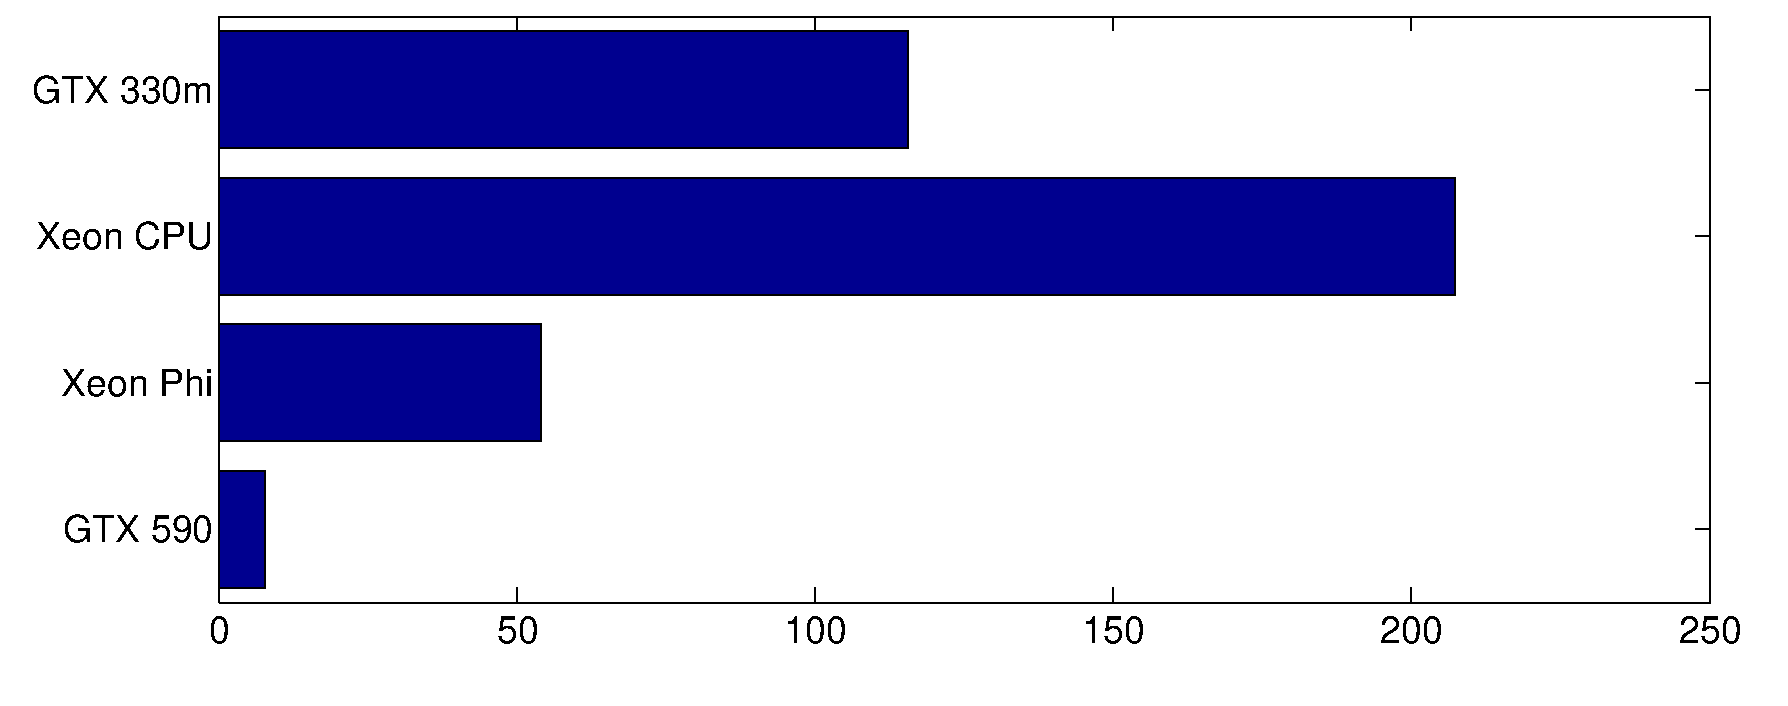
\includegraphics[width=0.9\columnwidth]{figures/eps/runtime.eps}
	  \caption{1000 kép feldolgozásának futási ideje [s]. A kissebb érték a kedvezőbb.}
	  \label{fig:runtime}
	\end{center}
	\end{figure}
	
	Az eszközök architekturájából fakadó különbségek számszerűsítése végett a futási időt egy compute-unitra és egy
	órajelre fajlagosan számítom:
	\begin{equation}
	T_{\rm fajl} = T \cdot N_{\rm CU} \cdot f_{\rm dev}
	\end{equation}
	ahol $T$ a futási idő $N_{\rm CU}$ az eszköz compute-unit száma és $f_{\rm dev}$ az eszköz órajelének frekvenciája.
        
	\begin{table}[H]
	\footnotesize
	\centering
	
	\setlength{\extrarowheight}{3pt}
	\begin{tabular}{ l | r | r | r | r}
		 & GTX 330m & Xeon E5-1620 & Xeon PHI & GTX 590\\ \hline
		\texttt{MAX\_COMPUTE\_UNITS} & 6 & 8 & 224 & 16\\
		\texttt{MAX\_CLOCK\_FREQUENCY} & 1265 & 3000 & 1100 & 1225\\\hline\hline
		Futási idő $(T)$ & 114.1~s & 202.0~s & 52.7~s & 7.74~s\\
		Fajlagos futási idő $(T_{\rm fajl})$ & 0.86$\times 10^6$ & 4.85$\times 10^6$ & 13.00$\times 10^6$ & 0.15$\times 10^6$
	\end{tabular}
	
	\caption{Eszközök fajlagos futási idejének összehasonlítása}
	\label{table:results_f}
	\end{table}	
	
	%\usepackage{graphics} is needed for \includegraphics
	\begin{figure}[!h]
	\begin{center}
	  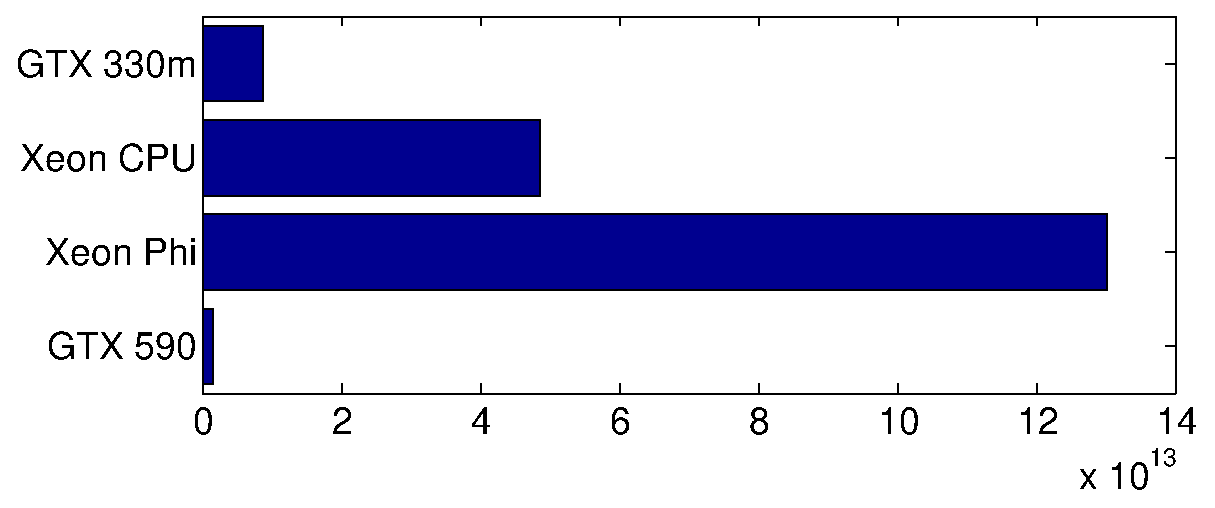
\includegraphics[width=0.9\columnwidth]{figures/eps/runtime_f.eps}
	  \caption{1000 kép feldolgozásának fajlagos futási ideje. A kissebb érték a kedvezőbb.}
	  \label{fig:runtime_f}
	\end{center}
	\end{figure}
	
	A program OpenCL-ben készült, így videokártyán és processzoron is tud futni.
	Ezt a GPU-k lokális memóriájának és annak programozott ``cache" működésének pozitív hatásának tudom be.
	
	A \ref{fig:runtime}.ábrát és a \ref{fig:runtime_f}. ábrát összevetve megfigyelhető, hogy a processzorok/processzorkártyák bár
	gyorsabban futtatják a programot, viszont ezt nagy fajlagos idővel teszik. Konklúzióként elmondható, hogy a program
	algoritmusához az architektúrájuk nem illeszkedik.
	


%----------------------------------------------------------------------------
\chapter{Összegzés}
%----------------------------------------------------------------------------
\cbstart
	Dolgozatomban bemutattam a porosplazma kísérletek apparátusát. A kísérlet során a kristályrácsba
	rendeződő részecskékről egy nagysebességű kamerával fényképek készülnek. A dolgozatomban ezen
	képeket, kellett feldolgoznom és a részecskék pozícióját detektálnom.
	A pozíciók a fizikai modell/szimuláció validálására szolgálnak.
	
	Ismertettem a részecske detektálásának módszerét szűrés és adaptív döntési küszöb használatával.
	Az elterjedt FIR Gauss szűrő helyett a hatékonyabb medián szűrőt javasoltam és alkalmaztam. A
	pozíció számítására a momentum módszert implementáltam, ami nagyobb számítási energiát igényel, de
	szubpixeles felbontást tudtam vele elérni. Konstatáltam, hogy az így kialakult program masszívan párhuzamosítható.
	
	Ezután áttekintettem az OpenCL keretrendszert, amit a párhuzamos program megírásának segítségére
	használtam. Az itt ismertetett megállapításokat figyelembe véve állítottam össze a párhuzamos
	program lépéseit, amit részleteztem is.
	
	Végül az elkészült programot CPU-n és GPU-n is futtatva a futási idejüket összevetettem és
	azonosítottam a gyorsulás forrását kitérve a processzormagra és a memóriájára.
	
	\section*{További feladatok:}
	\begin{itemize}
		\item A host-program real-time mérésbe helyezése egy producer-consumer sémájú szál megoldás
		alkalmazásával,
		\item Az eredmény grafikus  megjelenítése pl.: OpenGL használtatával,
		\item Az OpenCL szabvány által specifikált vektor műveletek támogatásának kiaknázása, ami az Intel
		Xeon PHI processzorkártyában rejlő teljesítményt ki tudná aknázni.
	\end{itemize}
	
\cbend

%----------------------------------------------------------------------------
\appendix
%----------------------------------------------------------------------------
\chapter*{Függelék}\addcontentsline{toc}{chapter}{Függelék}
\setcounter{chapter}{6}  % a fofejezet-szamlalo az angol ABC 6. betuje (F) lesz
\setcounter{equation}{0} % a fofejezet-szamlalo az angol ABC 6. betuje (F) lesz
\numberwithin{equation}{section}
\numberwithin{figure}{section}
\numberwithin{lstlisting}{section}
%\numberwithin{tabular}{section}
%----------------------------------------------------------------------------
%----------------------------------------------------------------------------
\chapter{Fejlesztőkörnyezet összeállítása}
%----------------------------------------------------------------------------

	OpenCL kód fejlesztése történhet Windows alatt NVIDIA Nsight Visual Studio
	Edition \cite{nsight} és Linux alatt GCC-vel \cite{gcc}.
	Az Open Source fejlesztőrendszer ingyenessége és az általa generált program hordozhatósága végett
	a Linux alatti fejlesztés mellett döntöttem. 
	Az OpenCL-t támogató hardverek legtöbbször CPU-k, GPU-k és az Intel MIC
	\cite{mic} kártyái.
	Ezekre való OpenCL kód fejlesztéséhez a gyártók biztosítanak Software Developement Kit-et (SDK).
	Ezek telepítése szinte bármelyik Linux disztribúción sikerülhet a megfelelő követelmények előzetes telepítése után.
	A Linux diszrók közül a CentOS-re \cite{centos} esett a választás, ami 
	csupán a fejlesztőkörnyezet egyszerűbb telepítése végett történt így.

\section{Software Developement Kit-ek (SDK) telepítése} \label{sect:sdk}
\subsection{nVidia támogatás telepítése}
	A legtöbb mai Linux disztrók tartalmaznak drivert az nVidia videó kártyákhoz.
	Ez az open source Nouveau, ami még nem támogatja az OpenCL-t.
	Így a hivatalos nVidia drivert fel kell telepítenünk.
	Ehhez először le kell tiltanunk a Nouveau betöltését.
	Ezt két helyen is meg kell tennünk: 
	egyrészt a \texttt{/etc/modprobe.d/blacklist.conf} fájlhoz hozzá kell adnunk a
	következő sort:
	\begin{lstlisting}
	blacklist nouveau
	\end{lstlisting}
	majd újragenerálni az INITial RAM File System-et (initramfs), ami a rendszer
	inicializásáért felelős:
	\begin{lstlisting}
	$ mv /boot/initramfs-$(uname -r).img /boot/initramfs-$(uname -r).img.bak
	$ dracut -v /boot/initramfs-$(uname -r).img $(uname -r)
	\end{lstlisting}
	másrészt a rendszer indító GRand Unified Bootloader-ben (GRUB) is le kell
	tiltani a betöltését a kernel opció alábbi paranccsal való kiegészítésével:
	\begin{lstlisting}
	nouveau.modeset=0
	\end{lstlisting}
	Továbbá a telepítéshez szükséges követelményeket a következő parancsokkal telepíthetjük:
	\begin{lstlisting}
	$ yum groupinstall "Development Tools"
	$ yum install kernel-devel kernel-headers dkms
	\end{lstlisting}
	Ekkor a rendszer újraindítása után készen állunk a hivatalos nVidia driver
	telepítésére. A drivert a következő linken lehet letölteni \cite{nvidia-driver}.
	A grafikus felületet a telepítés idejére le kell állítani az X grafikus
	kiszolgálót
	\begin{lstlisting}
	$ init 3
	\end{lstlisting}
	paranccsal, majd a konzolban telepíthető a driver, ami a legtöbb munkát elvégzi helyettünk. Ezután az
	\begin{lstlisting}
	$ init 5
	\end{lstlisting}
	paranccsal áttérhetünk a grafikus felületre, ahol a megfelelő környezeti változókat kiegészíthetjük.
	Legcélratörőbb, ha a \texttt{$\tilde{}$/.bashrc} fájlt módosítjuk és hozzáadjuk
	a következő sorokat:
	\begin{lstlisting}
	PATH=$PATH:$HOME/bin:/usr/local/cuda/bin
	export PATH
	
	CUDA_INSTALL_PATH=/usr/local/cuda
	export CUDA_INSTALL_PATH
	
	LD_LIBRARY_PATH=/usr/local/cuda/lib64:/opt/intel/opencl/bin
	export LD_LIBRARY_PATH
	
	NVSDKCOMPUTE_ROOT=/usr/local/cuda/lib64
	export NVSDKCOMPUTE_ROOT
	
	INTELOCLSDKROOT=/opt/intel/opencl
	export INTELOCLSDKROOT
	\end{lstlisting}
	Mivel az nVidia limitálja a kernel futási időt 5 másodpercben limitálja,
	hosszabb kernel futási idő esetén a rendszer lefagy.
	Ezt a korlátozást a \texttt{/etc/X11/xorg.conf} fájl \texttt{Device} részének a
	következővel való kiegészítésével érhetjük el:
	\begin{lstlisting}
	Option "Interactive" "boolean"
	\end{lstlisting}
	Érvényre juttatásához az X újraindítása szükséges (CTRL+ALT+Backspace).
	Ezután nagyobb problémák esetén már nem fogja lefagyasztani a rendszert a
	watchdog.

\subsection{Intel támogatás telepítése}
	A következő oldalról letölthetjük az SDK-t \cite{intel-sdk}.
	A kicsomagolás után az \texttt{./install-cpu.sh} program futtatásával
	telepíthető.
	Ezután még szükséges a \texttt{LD\_LIBRARY\_PATH} beállítása.

\subsection{Eclipse – Integrated Developement Environment}
	A fejlesztés és hibakeresés egy Integrated Developement Enviroment (IDE)
	segítségével könnyebb.
	Az open source Eclipse \cite{eclipse} fejlesztőkörnyezet a különböző pluginjaival épp
	megfelelő erre a célra.
	Például a C-nyelv fejlesztését segítő C/C++ Developement Tooling (CDT),
	a verziókövetést menedzselő EGit és a hibakeresést támogató GDT.
	A sok Eclipse változat közül az OpenCL fejlesztéshez legjobban az
	Eclipse for Parallel Application Developers verzió illik, mivel a korábban említett pluginokat már eleve tartalmazza.


\section{Új (Hello World) projekt létrehozása}
	Az OpenCL fejlesztését konyhanyelven bemutató OpenCL Programming Guide \cite{Munshi2011}
	könyvben szereplő Hello World programot a következő linken lehet letölteni
	\cite{hellow}.
	A kód fordítása elött egy Eclipse projektet létrehozunk és a
	fordításhoz szükséges beállításokat elvégezzük.

\subsection{Empty C project létrehozása}
	Először egy üres C projektet hozunk létre, ami folyamatát a \ref{fig:newproj} 
	ábrán látjuk. A korábban említettek szerint fordítónak a Linux GCC-t
	állítjuk be.
	\begin{figure}[H]
	\centering
	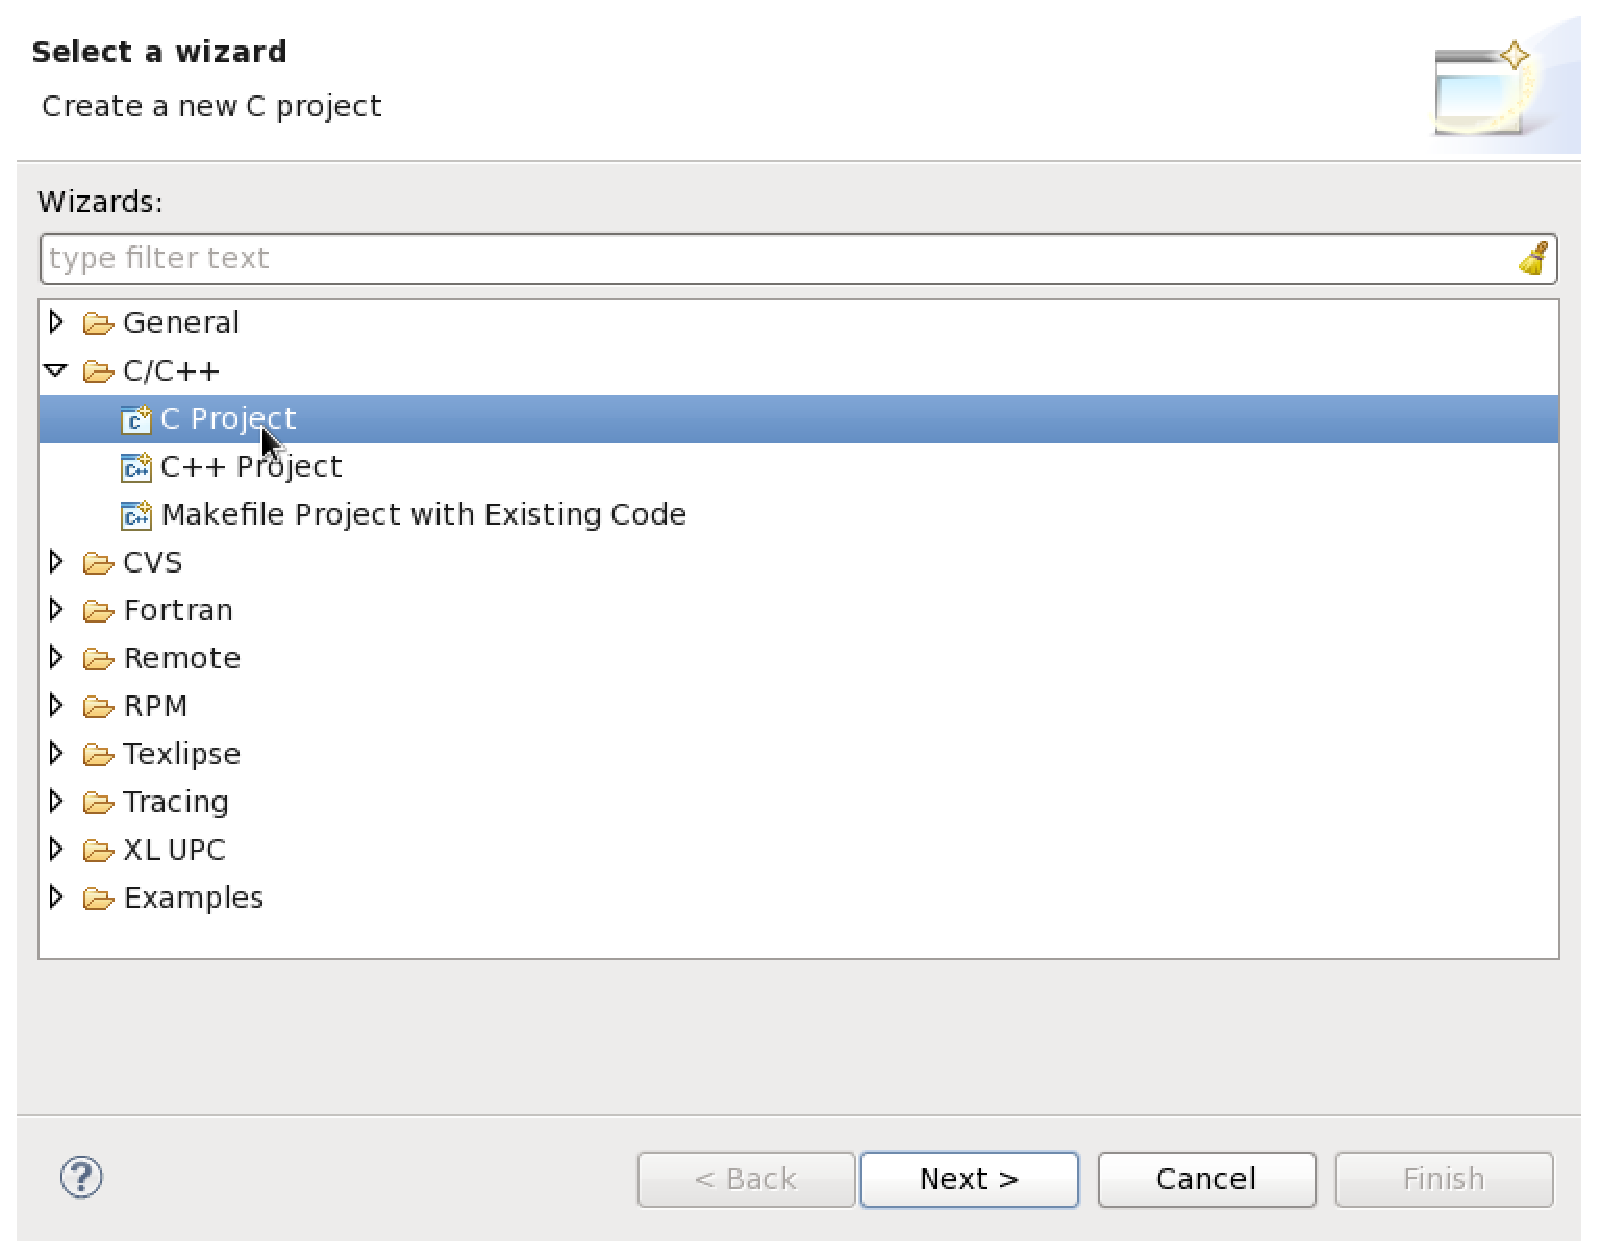
\includegraphics[width=67mm, keepaspectratio]{figures/eps/newC.eps}\hspace{1cm}
	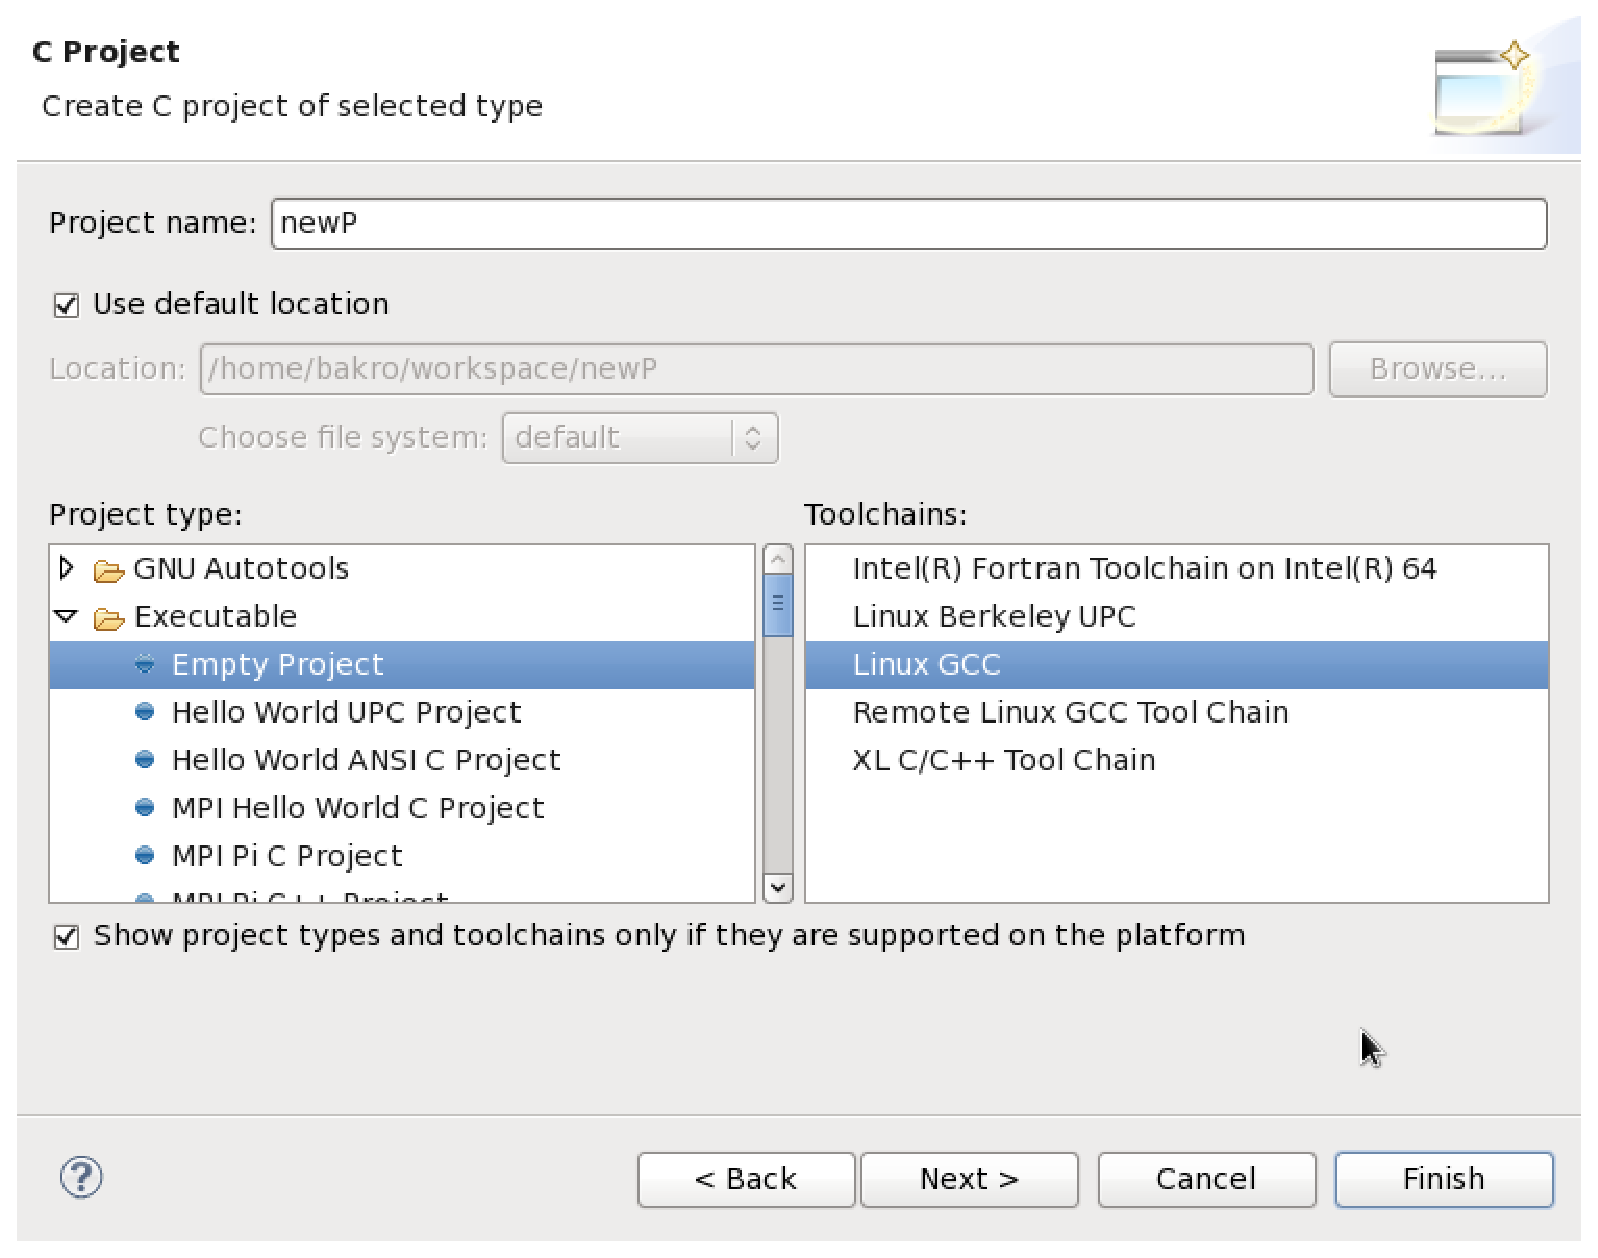
\includegraphics[width=67mm, keepaspectratio]{figures/eps/newP.eps}\\\vspace{5mm}
	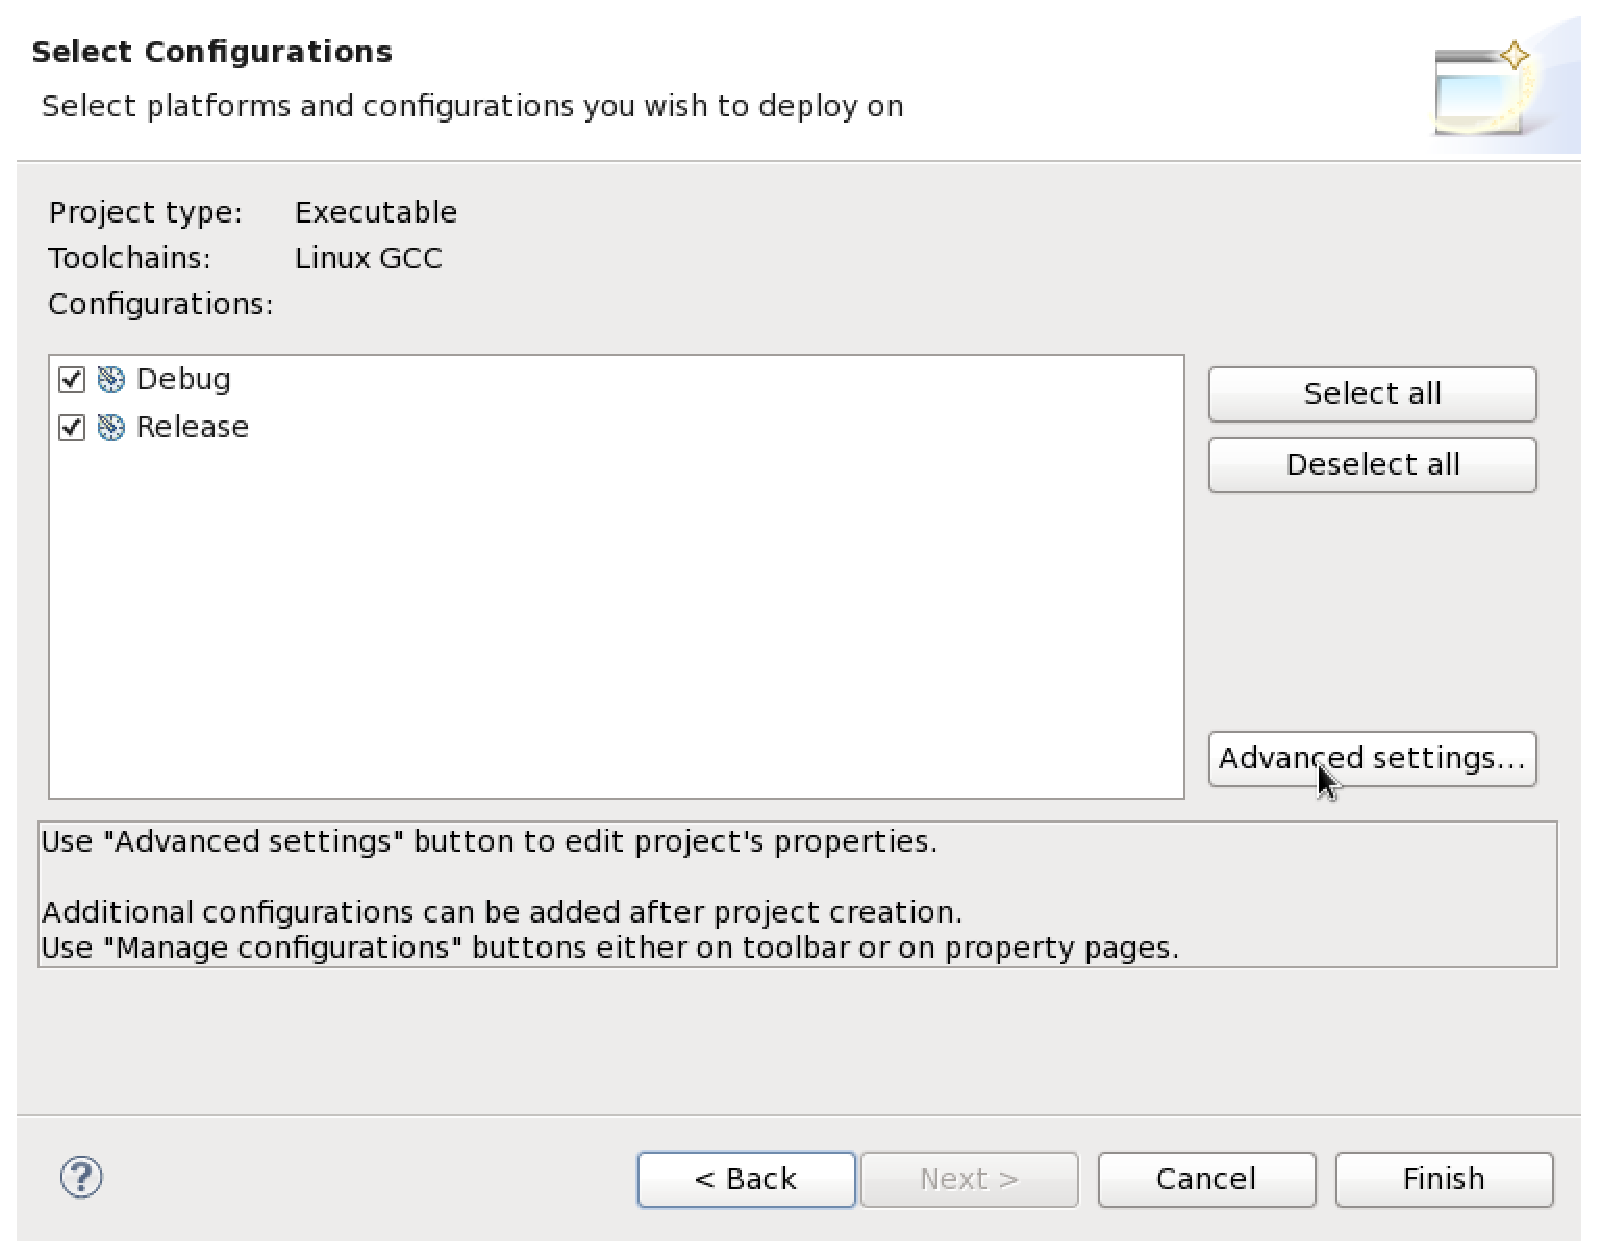
\includegraphics[width=67mm, keepaspectratio]{figures/eps/conf.eps}\hspace{1cm}
	\caption{Új Eclipse projekt létrehozása} 
	\label{fig:newproj}
	\end{figure}

\subsection{Compiler beállítása}
	A létrehozott projektre jobb gombbal kattíntva a tulajdonságára kattintva
	állíthatjuk be a fordítót a képnek \ref{fig:compiler} megfelelően.
	A beállítások kiterjednek a GNU-C99 nyelv szerinti fordításra és a korábbi
	\ref{sect:sdk} részben telepített SDK-ban található include mappa beállítására. 
	\begin{figure}[H]
	\centering
	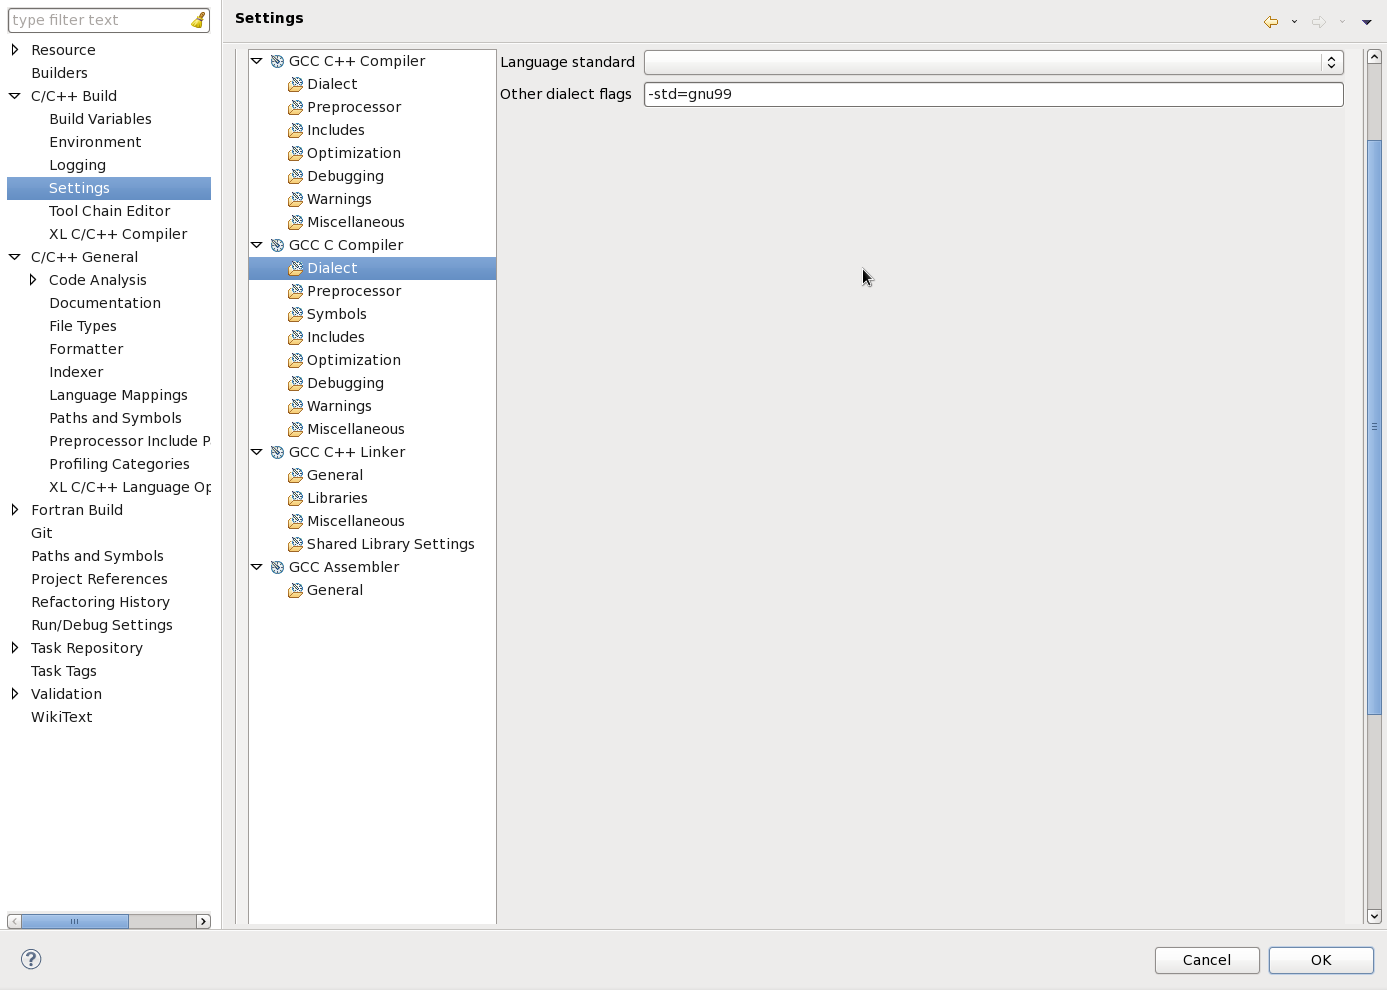
\includegraphics[width=67mm, keepaspectratio]{figures/eps/lang.eps}\hspace{1cm}
	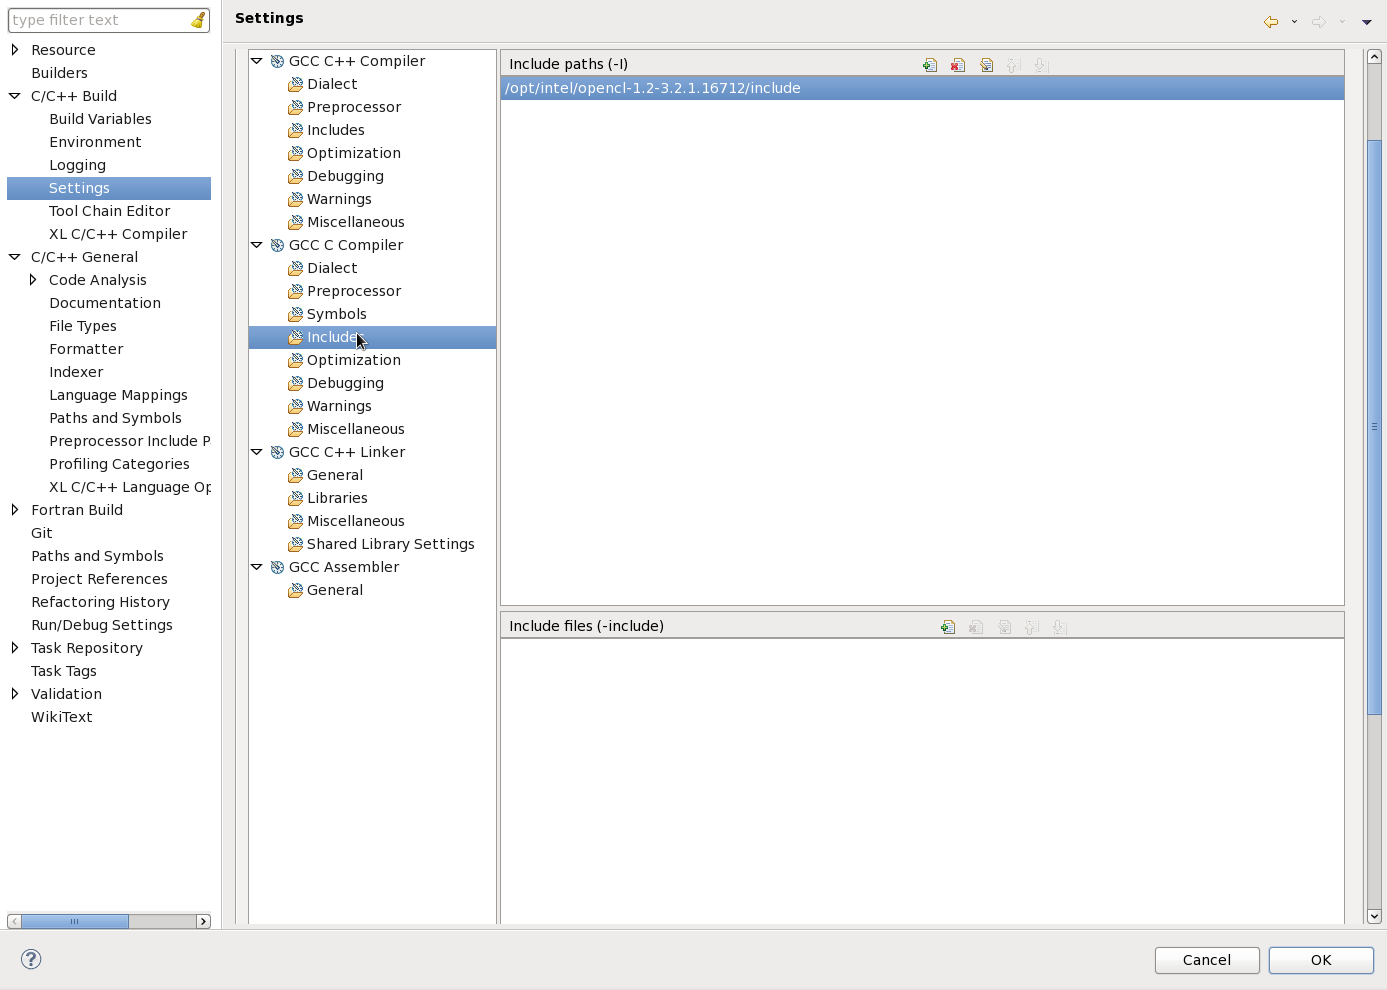
\includegraphics[width=67mm, keepaspectratio]{figures/eps/include.eps}\\\vspace{5mm}
	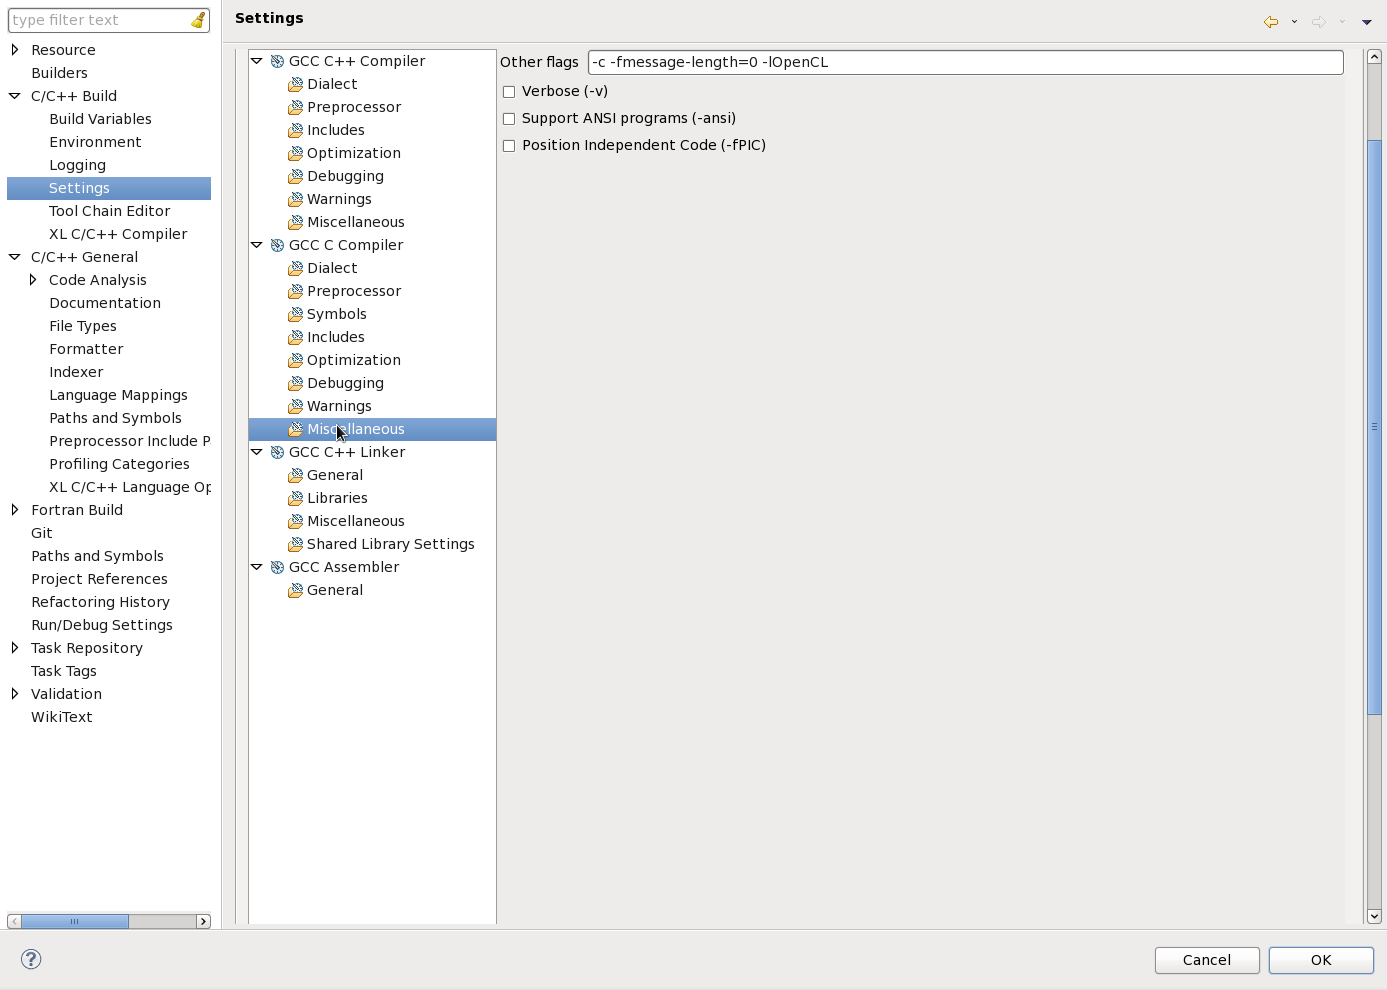
\includegraphics[width=67mm, keepaspectratio]{figures/eps/misc.eps}
	\caption{Compiler beállításai} 
	\label{fig:compiler}
	\end{figure}

\subsection{Linker beállítása}
	A linkert a \ref{fig:linker} ábra szerint állítjuk be.
	\begin{figure}[H]
	\centering
	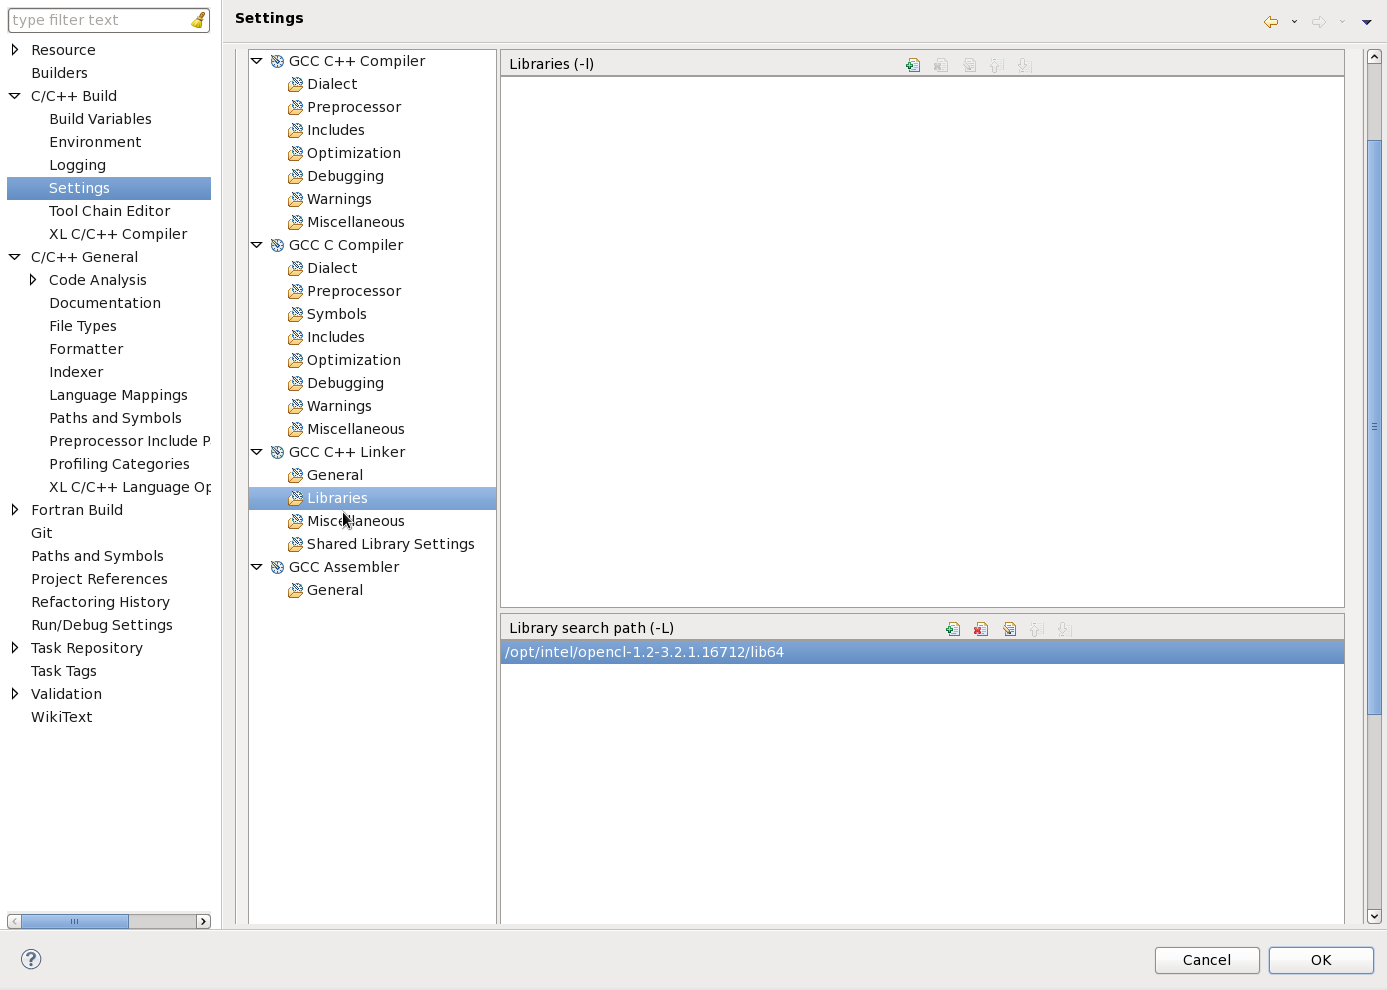
\includegraphics[width=67mm, keepaspectratio]{figures/eps/link.eps}\hspace{1cm}
	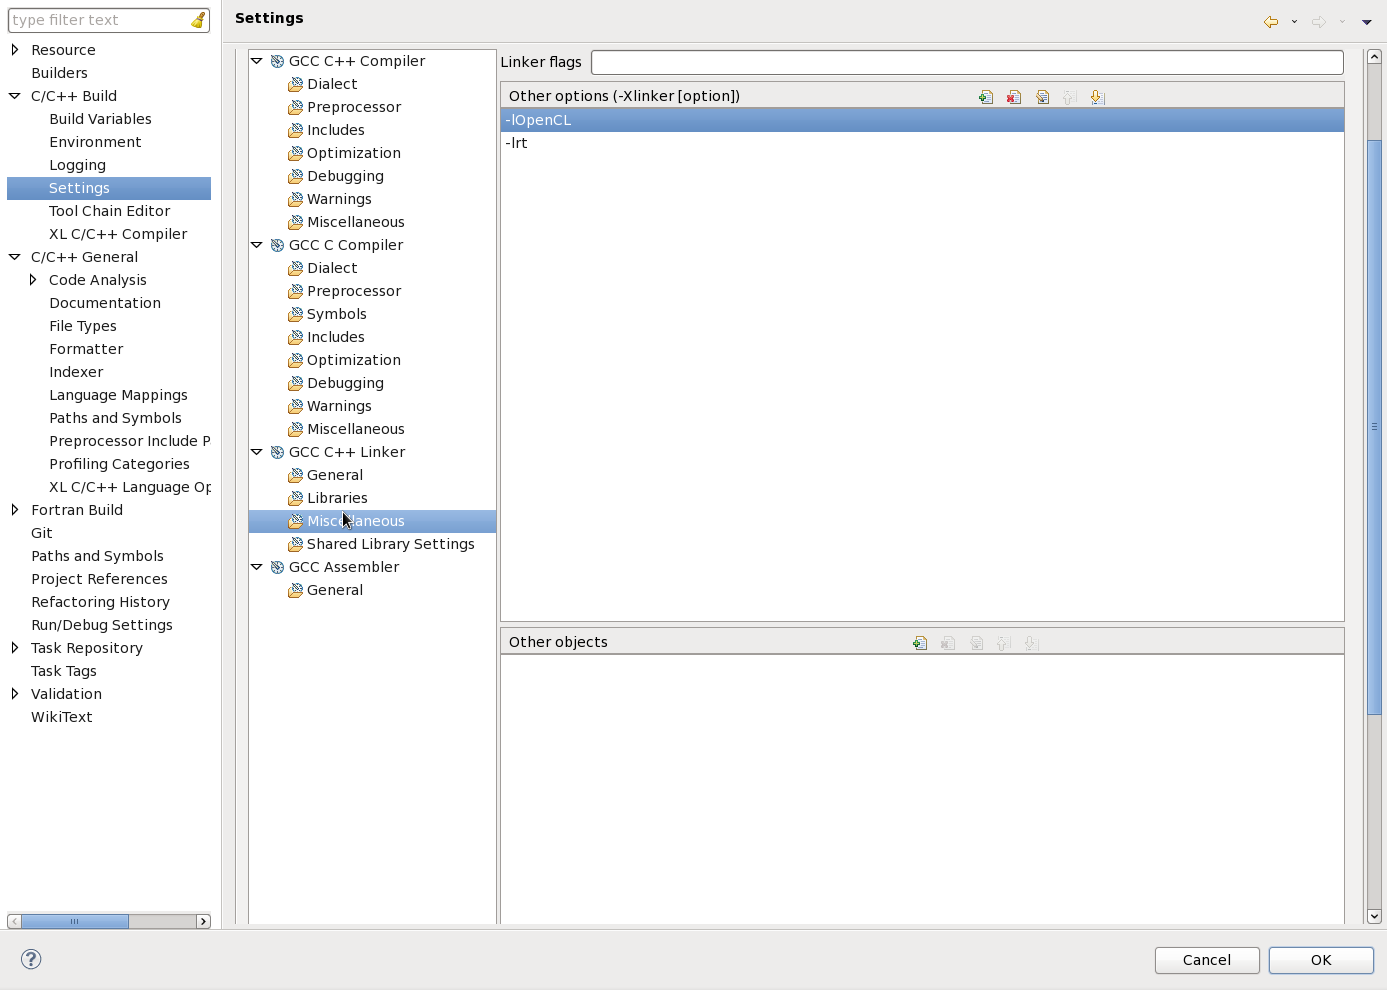
\includegraphics[width=67mm, keepaspectratio]{figures/eps/link_misc.eps}\\\vspace{5mm}
	\caption{Linker beállításai} 
	\label{fig:linker}
	\end{figure}



\cleartorightpage
\pagenumbering{Roman}
\setcounter{page}{1}

\listoffigures	\addcontentsline{toc}{chapter}{Ábrák jegyzéke}
\listoftables	\addcontentsline{toc}{chapter}{Táblázatok jegyzéke}

\bibliography{diploma1.bib} \addcontentsline{toc}{chapter}{Irodalomjegyzék}
\bibliographystyle{ieeetr}


\label{page:last}
\end{document}
